\documentclass[11pt, letterpaper]{article}
\usepackage[margin=1in]{geometry}
\usepackage{booktabs}
\usepackage{array}
\usepackage{tabularx}
\usepackage[table]{xcolor}
\usepackage{multirow}
\usepackage{enumitem}
\usepackage{titlesec}
\usepackage[hidelinks]{hyperref}
\usepackage{amsmath}
\usepackage{amssymb}
\usepackage[expansion=false]{microtype}
\usepackage{tcolorbox}
\usepackage{multicol}
\usepackage{titletoc}
\usepackage{needspace}
\usepackage{tikz}
\usepackage{pgfplots}
\pgfplotsset{compat=1.16}
\usetikzlibrary{arrows.meta, positioning, calc, shapes.geometric, decorations.markings}

\tcbuselibrary{skins, breakable}

\definecolor{sectionblue}{RGB}{30, 90, 160}
\definecolor{sectiongreen}{RGB}{30, 130, 80}
\definecolor{sectionpurple}{RGB}{100, 40, 140}
\definecolor{sectionorange}{RGB}{180, 90, 20}
\definecolor{sectionteal}{RGB}{20, 120, 120}
\definecolor{sectionred}{RGB}{160, 30, 40}
\definecolor{sectiongrey}{RGB}{70, 70, 70}
\definecolor{tableheader}{RGB}{220, 230, 245}
\definecolor{tableheadergreen}{RGB}{210, 240, 220}
\definecolor{tableheaderorange}{RGB}{255, 235, 210}
\definecolor{tableheaderteal}{RGB}{210, 240, 240}
\definecolor{tableheaderred}{RGB}{250, 220, 222}
\definecolor{tableheaderpurple}{RGB}{235, 220, 245}
\definecolor{tableheadergrey}{RGB}{230, 230, 230}
\definecolor{rowA}{RGB}{252, 252, 252}
\definecolor{rowB}{RGB}{237, 244, 255}
\definecolor{rowBg}{RGB}{237, 248, 241}
\definecolor{rowOr}{RGB}{255, 245, 232}
\definecolor{rowTe}{RGB}{232, 248, 248}
\definecolor{rowPu}{RGB}{245, 235, 255}
\definecolor{rowRe}{RGB}{255, 238, 238}
\definecolor{rowGr}{RGB}{242, 242, 242}
\definecolor{partbg}{RGB}{240, 244, 255}
\definecolor{part2bg}{RGB}{240, 252, 244}
\definecolor{part3bg}{RGB}{248, 240, 255}
\definecolor{part4bg}{RGB}{255, 245, 232}
\definecolor{part5bg}{RGB}{232, 248, 248}
\definecolor{part6bg}{RGB}{255, 240, 240}
\definecolor{part7bg}{RGB}{242, 242, 242}
\definecolor{notebg}{RGB}{255, 252, 228}
\definecolor{noteborder}{RGB}{180, 148, 30}
\definecolor{examplebg}{RGB}{240, 248, 255}
\definecolor{exampleborder}{RGB}{60, 100, 160}
\definecolor{warnbg}{RGB}{255, 240, 240}
\definecolor{warnborder}{RGB}{180, 40, 40}

\newcommand{\bluesections}{%
  \titleformat{\section}{\large\bfseries\color{sectionblue}}{}{0em}{}[\color{sectionblue}\titlerule]%
  \titleformat{\subsection}{\normalsize\bfseries\color{sectionblue!80!black}}{}{0em}{}%
}
\newcommand{\greensections}{%
  \titleformat{\section}{\large\bfseries\color{sectiongreen}}{}{0em}{}[\color{sectiongreen}\titlerule]%
  \titleformat{\subsection}{\normalsize\bfseries\color{sectiongreen!80!black}}{}{0em}{}%
}
\newcommand{\purplesections}{%
  \titleformat{\section}{\large\bfseries\color{sectionpurple}}{}{0em}{}[\color{sectionpurple}\titlerule]%
  \titleformat{\subsection}{\normalsize\bfseries\color{sectionpurple!80!black}}{}{0em}{}%
}
\newcommand{\orangesections}{%
  \titleformat{\section}{\large\bfseries\color{sectionorange}}{}{0em}{}[\color{sectionorange}\titlerule]%
  \titleformat{\subsection}{\normalsize\bfseries\color{sectionorange!80!black}}{}{0em}{}%
}
\newcommand{\tealsections}{%
  \titleformat{\section}{\large\bfseries\color{sectionteal}}{}{0em}{}[\color{sectionteal}\titlerule]%
  \titleformat{\subsection}{\normalsize\bfseries\color{sectionteal!80!black}}{}{0em}{}%
}
\newcommand{\redsections}{%
  \titleformat{\section}{\large\bfseries\color{sectionred}}{}{0em}{}[\color{sectionred}\titlerule]%
  \titleformat{\subsection}{\normalsize\bfseries\color{sectionred!80!black}}{}{0em}{}%
}
\newcommand{\greysections}{%
  \titleformat{\section}{\large\bfseries\color{sectiongrey}}{}{0em}{}[\color{sectiongrey}\titlerule]%
  \titleformat{\subsection}{\normalsize\bfseries\color{sectiongrey!80!black}}{}{0em}{}%
}

\newcommand{\partbanner}[3]{%
  \begin{tcolorbox}[colback=#1, colframe=#2, boxrule=1.2pt, arc=4pt,
    left=8pt, right=8pt, top=6pt, bottom=6pt]
    \begin{center}{\LARGE\bfseries #3}\end{center}
  \end{tcolorbox}%
}

\newcommand{\example}[1]{%
  \begin{tcolorbox}[colback=examplebg, colframe=exampleborder,
    title={\bfseries Example}, arc=3pt, boxrule=1pt]
  #1
  \end{tcolorbox}%
}

\newcommand{\warning}[1]{%
  \begin{tcolorbox}[colback=warnbg, colframe=warnborder,
    title={\bfseries Watch Out}, arc=3pt, boxrule=1pt]
  #1
  \end{tcolorbox}%
}

\setlength{\parskip}{4pt}
\setlength{\parindent}{0pt}
\hbadness=10000
\hfuzz=5pt

\setcounter{tocdepth}{2}
\setcounter{secnumdepth}{0}

\titlecontents{section}[1.5em]{\smallskip}
  {\contentslabel{1.5em}}{\hspace*{-1.5em}}
  {\titlerule*[6pt]{.}\contentspage}
\titlecontents{subsection}[3.5em]{}
  {\contentslabel{2em}}{\hspace*{-2em}}
  {\titlerule*[6pt]{.}\contentspage}

% Each topic has its own clickable table-of-contents destination.
\newcommand{\reftopic}[1]{%
  \phantomsection\addcontentsline{toc}{subsection}{#1}%
  \section*{#1}%
}
\newcommand{\refdetail}[1]{%
  \phantomsection\addcontentsline{toc}{subsubsection}{#1}%
  \subsection*{#1}%
}
\setcounter{tocdepth}{3}

\begin{document}

\begin{center}
  {\Huge\bfseries Calculus \& Precalculus Reference}\\[6pt]
  {\large Foundations, Trigonometry, Limits, Differentiation \& Integration}\\[4pt]
  \rule{\textwidth}{0.8pt}
\end{center}
\vspace{8pt}
\tableofcontents
\clearpage

%% =============================================================================
%%  PART I -- The Number System
%% =============================================================================
\purplesections
\phantomsection
\addcontentsline{toc}{section}{\textcolor{sectionpurple}{PART I \textemdash\ The Number System}}
\partbanner{part3bg}{sectionpurple}{Part I \quad The Number System}

\vspace{6pt}
\begin{center}\small\itshape
  Before calculus, you need to know exactly what kind of ``number'' you're working with.
  Every number lives inside a nested hierarchy of sets.
\end{center}

\reftopic{The Hierarchy of Numbers}

Every number belongs to progressively narrower categories. The largest set is Complex Numbers; the smallest, most familiar set is Natural Numbers.

\begin{center}
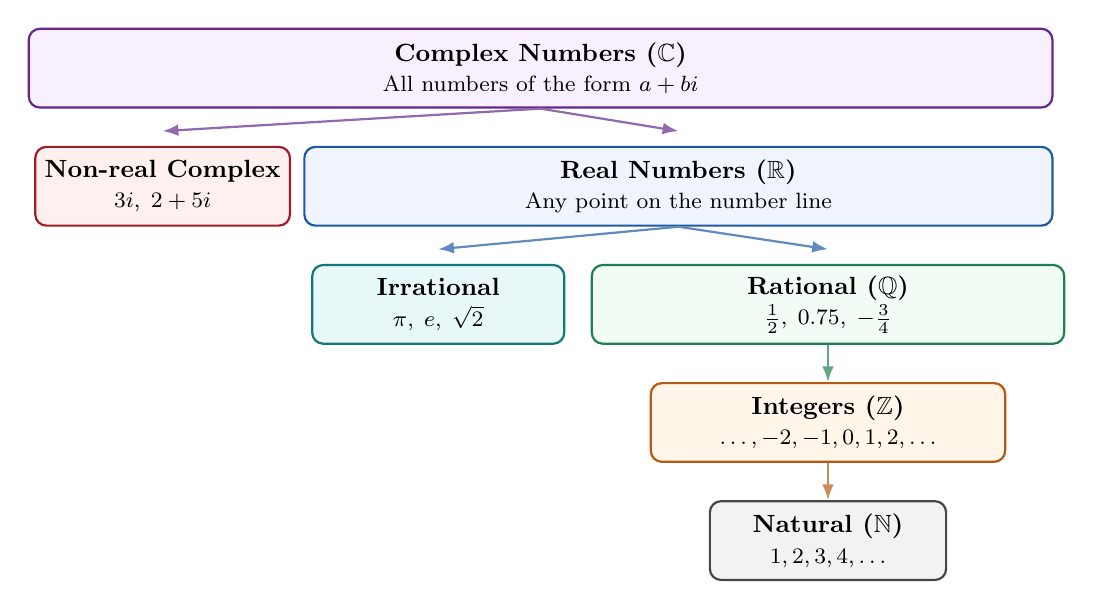
\begin{tikzpicture}[
  every node/.style={rounded corners=4pt, align=center, font=\small},
  complex/.style={draw=sectionpurple, fill=part3bg, thick, minimum width=13cm, minimum height=1cm},
  real/.style={draw=sectionblue, fill=partbg, thick, minimum width=9.5cm, minimum height=1cm},
  imag/.style={draw=sectionred, fill=part6bg, thick, minimum width=3.2cm, minimum height=1cm},
  irr/.style={draw=sectionteal, fill=part5bg, thick, minimum width=3.2cm, minimum height=1cm},
  rat/.style={draw=sectiongreen, fill=part2bg, thick, minimum width=6cm, minimum height=1cm},
  intg/.style={draw=sectionorange, fill=part4bg, thick, minimum width=4.5cm, minimum height=1cm},
  nat/.style={draw=sectiongrey, fill=part7bg, thick, minimum width=3cm, minimum height=1cm}
]
\node[complex] (C) at (0, 5) {\textbf{Complex Numbers ($\mathbb{C}$)} \\ \footnotesize All numbers of the form $a + bi$};
\node[imag] (I) at (-4.8, 3.5) {\textbf{Non-real Complex} \\ \footnotesize $3i, \; 2+5i$};
\node[real] (R) at (1.75, 3.5) {\textbf{Real Numbers ($\mathbb{R}$)} \\ \footnotesize Any point on the number line};
\node[irr] (Irr) at (-1.3, 2.0) {\textbf{Irrational} \\ \footnotesize $\pi, \; e, \; \sqrt{2}$};
\node[rat] (Q) at (3.65, 2.0) {\textbf{Rational ($\mathbb{Q}$)} \\ \footnotesize $\tfrac{1}{2}, \; 0.75, \; -\tfrac{3}{4}$};
\node[intg] (Z) at (3.65, 0.5) {\textbf{Integers ($\mathbb{Z}$)} \\ \footnotesize $\ldots, -2, -1, 0, 1, 2, \ldots$};
\node[nat] (N) at (3.65, -1.0) {\textbf{Natural ($\mathbb{N}$)} \\ \footnotesize $1, 2, 3, 4, \ldots$};

\draw[-{Latex[length=2mm]}, thick, sectionpurple!70] (C.south) -- (-4.8, 4.2);
\draw[-{Latex[length=2mm]}, thick, sectionpurple!70] (C.south) -- (1.75, 4.2);
\draw[-{Latex[length=2mm]}, thick, sectionblue!70] (R.south) -- (-1.3, 2.7);
\draw[-{Latex[length=2mm]}, thick, sectionblue!70] (R.south) -- (3.65, 2.7);
\draw[-{Latex[length=2mm]}, thick, sectiongreen!70] (Q.south) -- (Z.north);
\draw[-{Latex[length=2mm]}, thick, sectionorange!70] (Z.south) -- (N.north);
\end{tikzpicture}
\end{center}

\reftopic{The Filtering Rules}

To figure out where any number lands, apply these filters in order:

\begin{tcolorbox}[colback=part3bg, colframe=sectionpurple, arc=3pt, boxrule=1pt]
\textbf{1. The Imaginary Filter (Real vs.\ Complex):} After simplification, does the number have a nonzero imaginary part?
\begin{itemize}[noitemsep, leftmargin=*]
  \item \textbf{YES} $\to$ Non-real complex ($4i$, $3 + 2i$). Used when solving equations like $x^2 + 1 = 0$.
  \item \textbf{NO} $\to$ Real Number ($\mathbb{R}$). Lives somewhere on a continuous 1D number line.
\end{itemize}

\textbf{2. The Fraction Filter (Rational vs.\ Irrational):} Can it be written as $\frac{a}{b}$ (both integers)?
\begin{itemize}[noitemsep, leftmargin=*]
  \item \textbf{NO} $\to$ Irrational. Infinite, non-repeating decimals ($\pi \approx 3.14159\ldots$, $e$, $\sqrt{2}$).
  \item \textbf{YES} $\to$ Rational ($\mathbb{Q}$). Terminating or repeating ($\tfrac{1}{2}$, $0.\overline{3} = \tfrac{1}{3}$, $4 = \tfrac{4}{1}$).
\end{itemize}

\textbf{3. The Whole Number Filter (Integer or not):} Does it have a fractional part?
\begin{itemize}[noitemsep, leftmargin=*]
  \item \textbf{YES} $\to$ Stays a rational fraction ($2.5$, $-\tfrac{3}{4}$).
  \item \textbf{NO} $\to$ Integer ($\mathbb{Z}$). No decimals; positive or negative ($-5, -1, 0, 3, 42$).
\end{itemize}

\textbf{4. The Sign/Zero Filter (Natural / Counting):} Is it positive and non-zero?
\begin{itemize}[noitemsep, leftmargin=*]
  \item \textbf{NO} $\to$ Negative integer or zero.
  \item \textbf{YES} $\to$ Natural Number ($\mathbb{N}$). Basic counting: $1, 2, 3, \ldots$
\end{itemize}
\end{tcolorbox}

\reftopic{Mathematical Symbols Reference}

\subsection*{Arithmetic Operators}

\noindent
{\renewcommand{\arraystretch}{1.5}
\begin{tabularx}{\textwidth}{>{\centering\arraybackslash}p{1.5cm}
                              >{\bfseries\raggedright\arraybackslash}p{3cm}
                              >{\raggedright\arraybackslash}X}
\toprule
\rowcolor{tableheaderpurple}
\textbf{Symbol} & \textbf{Name} & \textbf{Meaning / Usage} \\
\midrule
\rowcolor{rowPu} $+ \; / \; -$ & Plus / Minus & Addition and subtraction. \\
\rowcolor{rowA}  $\cdot \; / \; \times$ & Multiply & Multiplication ($3 \cdot x$ or $3 \times x$). \\
\rowcolor{rowPu} $\div \; / \; /$ & Divide & Division ($a / b$). \\
\rowcolor{rowA}  $\pm$ & Plus-Minus & Both values (quadratic formula: $3 \pm 2$). \\
\rowcolor{rowPu} $!$ & Factorial & $5! = 5 \cdot 4 \cdot 3 \cdot 2 \cdot 1 = 120$. \\
\rowcolor{rowA}  $\sqrt{x}$ & Square Root & Number that squared gives $x$ ($\sqrt{9} = 3$). \\
\rowcolor{rowPu} $\sqrt[n]{x}$ & $n$-th Root & $\sqrt[3]{8} = 2$. \\
\rowcolor{rowA}  $|x|$ & Absolute Value & Distance from zero ($|{-5}| = 5$). \\
\bottomrule
\end{tabularx}}

\subsection*{Relations \& Comparison}

\noindent
{\renewcommand{\arraystretch}{1.5}
\begin{tabularx}{\textwidth}{>{\centering\arraybackslash}p{1.5cm}
                              >{\bfseries\raggedright\arraybackslash}p{3.5cm}
                              >{\raggedright\arraybackslash}X}
\toprule
\rowcolor{tableheaderpurple}
\textbf{Symbol} & \textbf{Name} & \textbf{Meaning / Usage} \\
\midrule
\rowcolor{rowPu} $=$ & Equals & Exact equality ($x = 5$). \\
\rowcolor{rowA}  $\neq$ & Not Equal & $x \neq 2$ (domain restrictions/holes). \\
\rowcolor{rowPu} $\approx$ & Approximately Equal & Rounded estimate ($\pi \approx 3.14$). \\
\rowcolor{rowA}  $\equiv$ & Identically Equal & True for all inputs ($x + x \equiv 2x$). \\
\rowcolor{rowPu} $<$ / $>$ & Less / Greater Than & Strict inequalities. \\
\rowcolor{rowA}  $\leq$ / $\geq$ & Less/Greater or Equal & Non-strict (real radical domains). \\
\rowcolor{rowPu} $\infty$ & Infinity & Unbounded growth (not a number). \\
\bottomrule
\end{tabularx}}

\subsection*{Algebra, Sets \& Logic}

\noindent
{\renewcommand{\arraystretch}{1.5}
\begin{tabularx}{\textwidth}{>{\centering\arraybackslash}p{1.5cm}
                              >{\bfseries\raggedright\arraybackslash}p{3.5cm}
                              >{\raggedright\arraybackslash}X}
\toprule
\rowcolor{tableheaderpurple}
\textbf{Symbol} & \textbf{Name} & \textbf{Meaning / Usage} \\
\midrule
\rowcolor{rowPu} $\in$ & Element Of & $x \in \mathbb{R}$: ``$x$ is a real number.'' \\
\rowcolor{rowA}  $\notin$ & Not Element Of & Does not belong to the set. \\
\rowcolor{rowPu} $\mathbb{R}$ & Real Numbers & Rational + irrational. \\
\rowcolor{rowA}  $\mathbb{C}$ & Complex Numbers & $a + bi$ form. \\
\rowcolor{rowPu} $\mathbb{Z}$ & Integers & $\ldots, -2, -1, 0, 1, 2, \ldots$ \\
\rowcolor{rowA}  $\mathbb{Q}$ & Rationals & Fractions of integers. \\
\rowcolor{rowPu} $\mathbb{N}$ & Naturals & $1, 2, 3, \ldots$ \\
\rowcolor{rowA}  $\cup \; / \; \cap$ & Union / Intersection & Combine sets / find common elements. \\
\rowcolor{rowPu} $[a, b]$ & Closed Interval & Includes endpoints ($a \leq x \leq b$). \\
\rowcolor{rowA}  $(a, b)$ & Open Interval & Excludes endpoints ($a < x < b$). \\
\rowcolor{rowPu} $\implies$ & Implies & Logical ``if\ldots then\ldots'' \\
\rowcolor{rowA}  $\iff$ & If and Only If & Two-way logical equivalence. \\
\bottomrule
\end{tabularx}}

\subsection*{Calculus \& Limits}

\noindent
{\renewcommand{\arraystretch}{1.5}
\begin{tabularx}{\textwidth}{>{\centering\arraybackslash}p{2cm}
                              >{\bfseries\raggedright\arraybackslash}p{3.5cm}
                              >{\raggedright\arraybackslash}X}
\toprule
\rowcolor{tableheaderpurple}
\textbf{Symbol} & \textbf{Name} & \textbf{Meaning / Usage} \\
\midrule
\rowcolor{rowPu} $\lim_{x \to a}$ & Limit & Value $f(x)$ approaches as $x$ gets close to $a$. \\
\rowcolor{rowA}  $x \to a^+$ & Right-hand limit & Approaching $a$ from values greater than $a$. \\
\rowcolor{rowPu} $x \to a^-$ & Left-hand limit & Approaching $a$ from values less than $a$. \\
\rowcolor{rowA}  $\frac{dy}{dx}$ / $f'(x)$ & Derivative & Instantaneous rate of change / tangent slope. \\
\rowcolor{rowPu} $\int$ & Integral & Area under a curve (anti-derivative). \\
\rowcolor{rowA}  $\sum$ & Sigma (Summation) & Sum a sequence: $\sum_{i=1}^{n} i = 1+2+\ldots+n$. \\
\rowcolor{rowPu} $\Delta$ & Delta & Change in a variable ($\Delta x = x_2 - x_1$). \\
\bottomrule
\end{tabularx}}

\newpage

%% =============================================================================
%%  PART II -- Algebra Foundations
%% =============================================================================
\bluesections
\phantomsection
\addcontentsline{toc}{section}{\textcolor{sectionblue}{PART II \textemdash\ Algebra Foundations}}
\partbanner{partbg}{sectionblue}{Part II \quad Algebra Foundations}

\vspace{6pt}

\reftopic{Factoring Quadratics}

A \textbf{quadratic equation} has the standard form:
\[
  ax^2 + bx + c = 0
\]
The goal is to find the values of $x$ (called \textbf{roots} or \textbf{zeros}) that make the equation true. When possible, factoring is the fastest method.

\subsection*{Factoring by Grouping}

Find two numbers that multiply to $c$ and add to $b$. Split the middle term using them, then factor by grouping.

\example{
Solve $x^2 - 5x + 6 = 0$.\\[4pt]
Find factors of $c = 6$ that add to $b = -5$:
\[
(-2) \cdot (-3) = 6, \qquad (-2) + (-3) = -5 \; \checkmark
\]
Split the middle term:
\[
x^2 - 2x - 3x + 6 = 0
\]
Group and factor out the GCF from each pair:
\[
x(x - 2) - 3(x - 2) = 0
\]
\[
(x - 3)(x - 2) = 0
\]
Set each factor to zero:
\[
x - 3 = 0 \implies x = 3
\qquad\text{and}\qquad
x - 2 = 0 \implies x = 2
\]
\textbf{Solutions:} $x = 2$ and $x = 3$.
}

\reftopic{The Quadratic Formula}

When factoring is hard or impossible, the quadratic formula always works:
\[
  \boxed{\; x = \dfrac{-b \pm \sqrt{b^2 - 4ac}}{2a} \;}
\]

\example{
Solve $x^2 - 3x + 7 = 0$ using the quadratic formula. Here $a = 1$, $b = -3$, $c = 7$.\\[4pt]
Plug the coefficients into the formula:
\[
x = \frac{-(-3) \pm \sqrt{(-3)^2 - 4(1)(7)}}{2(1)}
= \frac{3 \pm \sqrt{9 - 28}}{2}
= \frac{3 \pm \sqrt{-19}}{2}
\]
Since the discriminant is negative, extract the imaginary unit $i = \sqrt{-1}$:
\[
x = \frac{3 \pm i\sqrt{19}}{2}
\]
Split into the two \textbf{complex roots}:
\[
x = \frac{3}{2} + \frac{\sqrt{19}}{2}i
\qquad\text{and}\qquad
x = \frac{3}{2} - \frac{\sqrt{19}}{2}i
\]
}

\reftopic{The Discriminant}

The expression under the square root, $b^2 - 4ac$, is called the \textbf{discriminant}. It tells you what kind of solutions to expect \emph{before} finishing the calculation.

\noindent
{\renewcommand{\arraystretch}{1.6}
\begin{tabularx}{\textwidth}{>{\centering\arraybackslash}p{3cm}
                              >{\bfseries\raggedright\arraybackslash}p{5cm}
                              >{\raggedright\arraybackslash}X}
\toprule
\rowcolor{tableheader}
\textbf{Discriminant} & \textbf{Type of Roots} & \textbf{What the graph looks like} \\
\midrule
\rowcolor{rowB} $b^2 - 4ac > 0$ & Two distinct real roots & Parabola crosses the $x$-axis at two points. \\
\rowcolor{rowA} $b^2 - 4ac = 0$ & One repeated real root  & Parabola just touches the $x$-axis at one point (vertex on axis). \\
\rowcolor{rowB} $b^2 - 4ac < 0$ & Two complex (imaginary) roots & Parabola does NOT cross the $x$-axis. \\
\bottomrule
\end{tabularx}}

\begin{tcolorbox}[colback=partbg, colframe=sectionblue, arc=3pt, boxrule=1pt]
\textbf{When to use which method:}
\begin{itemize}[noitemsep, leftmargin=*]
  \item \textbf{Try factoring first} when $a = 1$ and the numbers are small integers.
  \item \textbf{Use the quadratic formula} when factoring doesn't work, when the numbers are messy, or when you need the exact complex roots.
  \item \textbf{Check the discriminant first} if you only need to know how many real solutions exist.
\end{itemize}
\end{tcolorbox}

\newpage

%% =============================================================================
%%  PART III -- Complex Numbers & the Imaginary Unit
%% =============================================================================
\redsections
\phantomsection
\addcontentsline{toc}{section}{\textcolor{sectionred}{PART III \textemdash\ Complex Numbers \& the Imaginary Unit}}
\partbanner{part6bg}{sectionred}{Part III \quad Complex Numbers \& the Imaginary Unit}

\vspace{6pt}

\reftopic{The Imaginary Unit $i$}

In real numbers, you can't take the square root of a negative --- squaring any real number (positive or negative) gives a positive result: $2^2 = 4$ and $(-2)^2 = 4$.

To handle equations where $\sqrt{\text{negative}}$ appears, mathematicians defined the \textbf{imaginary unit}:
\[
  \boxed{\; i = \sqrt{-1} \qquad \text{so that} \qquad i^2 = -1 \;}
\]

\reftopic{The 4-Step Cycle of $i$}

Because $i^2 = -1$, powers of $i$ repeat every 4 steps.

\noindent
{\renewcommand{\arraystretch}{1.5}
\begin{tabularx}{\textwidth}{>{\centering\arraybackslash}p{2cm}
                              >{\centering\arraybackslash}p{4cm}
                              >{\raggedright\arraybackslash}X}
\toprule
\rowcolor{tableheaderred}
\textbf{Power} & \textbf{Simplification} & \textbf{Result} \\
\midrule
\rowcolor{rowRe} $i^1$ & $i$ & $i$ \\
\rowcolor{rowA}  $i^2$ & Definition & $-1$ \\
\rowcolor{rowRe} $i^3$ & $i^2 \cdot i = -1 \cdot i$ & $-i$ \\
\rowcolor{rowA}  $i^4$ & $i^2 \cdot i^2 = (-1)(-1)$ & $1$ \\
\rowcolor{rowRe} $i^5$ & $i^4 \cdot i = 1 \cdot i$ & $i$ \quad (cycle restarts) \\
\bottomrule
\end{tabularx}}

\textbf{Trick for large powers:} divide the exponent by 4 and use the remainder.
\begin{itemize}[noitemsep]
  \item Remainder 0 $\to$ $1$
  \item Remainder 1 $\to$ $i$
  \item Remainder 2 $\to$ $-1$
  \item Remainder 3 $\to$ $-i$
\end{itemize}
So $i^{27}$: $27 \div 4 = 6$ remainder $3$, so $i^{27} = -i$.

\reftopic{Simplifying Negative Square Roots}

Whenever a negative sits under a radical, split off the $-1$ and pull out an $i$:
\[
  \sqrt{-x} = \sqrt{x \cdot (-1)} = \sqrt{x} \cdot \sqrt{-1} = \sqrt{x} \cdot i
\]

\example{
\textbf{Simplify $\sqrt{-19}$:}
\[
\sqrt{-19} = \sqrt{19 \cdot (-1)} = \sqrt{19} \cdot \sqrt{-1} = \sqrt{19}\, i = i\sqrt{19}
\]
\textbf{Simplify $\sqrt{-25}$:}
\[
\sqrt{-25} = \sqrt{25} \cdot \sqrt{-1} = 5i
\]
}

\reftopic{Complex Number Operations}

A \textbf{complex number} combines a real part and an imaginary part:
\[
  z = a + bi
\]
where $a$ is the \textbf{real part} and $b$ is the \textbf{imaginary part}.

\textbf{Rule of thumb:} treat $i$ like a normal variable (like $x$), but replace $i^2$ with $-1$ whenever it appears.

\noindent
{\renewcommand{\arraystretch}{1.6}
\begin{tabularx}{\textwidth}{>{\bfseries\raggedright\arraybackslash}p{3cm}
                              >{\raggedright\arraybackslash}X}
\toprule
\rowcolor{tableheaderred}
\textbf{Operation} & \textbf{How it works (with example)} \\
\midrule
\rowcolor{rowRe} Addition & Add real parts and imaginary parts separately: \newline $(3 + 2i) + (1 + 4i) = (3+1) + (2+4)i = 4 + 6i$ \\
\rowcolor{rowA}  Subtraction & Same as addition but subtract: \newline $(5 + 3i) - (2 + 7i) = 3 - 4i$ \\
\rowcolor{rowRe} Multiplication (pure) & $(2i)(5i) = 10i^2 = 10(-1) = -10$ \\
\rowcolor{rowA}  Multiplication (FOIL) & $(1 + i)(2 + i)$: \newline $= 2 + i + 2i + i^2 = 2 + 3i + (-1) = 1 + 3i$ \\
\rowcolor{rowRe} Complex conjugate & The conjugate of $a + bi$ is $a - bi$. Multiplying gives a real number: $(a+bi)(a-bi) = a^2 + b^2$. \\
\bottomrule
\end{tabularx}}

\begin{tcolorbox}[colback=part6bg, colframe=sectionred, arc=3pt, boxrule=1pt]
\textbf{When do complex roots appear?} Whenever a quadratic has a \textbf{negative discriminant} ($b^2 - 4ac < 0$). The two roots always come as a \textbf{conjugate pair}: if $a + bi$ is a root, so is $a - bi$. This is why the roots of $x^2 - 3x + 7 = 0$ came out as $\tfrac{3}{2} \pm \tfrac{\sqrt{19}}{2}i$ --- a real part plus and minus an imaginary part.
\end{tcolorbox}

\newpage

%% =============================================================================
%%  PART IV -- Trigonometry & the Unit Circle
%% =============================================================================
\greensections
\phantomsection
\addcontentsline{toc}{section}{\textcolor{sectiongreen}{PART IV \textemdash\ Trigonometry \& the Unit Circle}}
\partbanner{part2bg}{sectiongreen}{Part IV \quad Trigonometry \& the Unit Circle}

\vspace{6pt}

\reftopic{Special Right Triangles}

Two right triangles show up constantly in trig. Memorize their side ratios.

\begin{center}
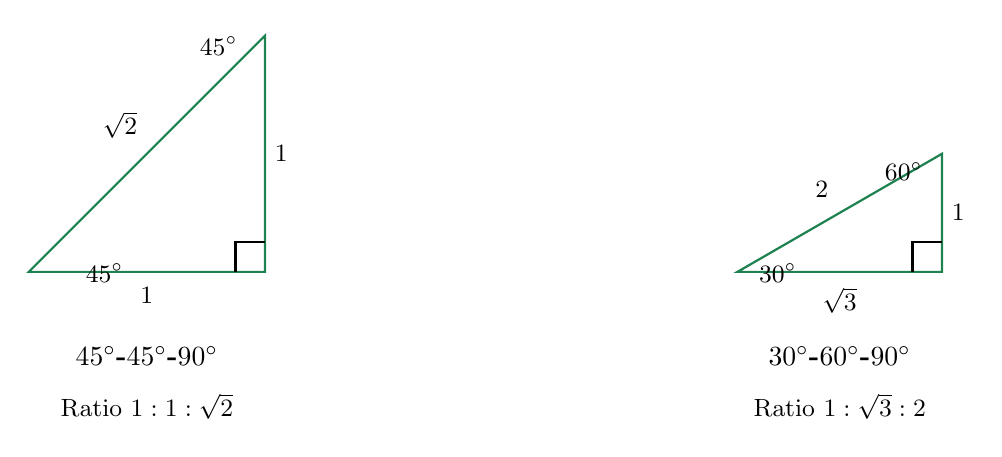
\begin{tikzpicture}[scale=1.5, every node/.style={font=\small}]
% 45-45-90 triangle
\begin{scope}[xshift=0cm]
  \draw[thick, sectiongreen] (0,0) -- (2,0) -- (2,2) -- cycle;
  \draw[thick] (1.75, 0) -- (1.75, 0.25) -- (2, 0.25);
  \node[below] at (1, -0.05) {$1$};
  \node[right] at (2, 1) {$1$};
  \node[above left] at (1, 1.05) {$\sqrt{2}$};
  \node[below right] at (0.4, 0.15) {$45^\circ$};
  \node[above left] at (1.85, 1.75) {$45^\circ$};
  \node[below, font=\bfseries] at (1, -0.55) {$45^\circ$-$45^\circ$-$90^\circ$};
  \node[below] at (1, -0.95) {Ratio $1 : 1 : \sqrt{2}$};
\end{scope}
% 30-60-90 triangle
\begin{scope}[xshift=6cm]
  \draw[thick, sectiongreen] (0,0) -- (1.732, 0) -- (1.732, 1) -- cycle;
  \draw[thick] (1.482, 0) -- (1.482, 0.25) -- (1.732, 0.25);
  \node[below] at (0.866, -0.05) {$\sqrt{3}$};
  \node[right] at (1.732, 0.5) {$1$};
  \node[above left] at (0.85, 0.55) {$2$};
  \node[below right] at (0.1, 0.15) {$30^\circ$};
  \node[left] at (1.65, 0.85) {$60^\circ$};
  \node[below, font=\bfseries] at (0.866, -0.55) {$30^\circ$-$60^\circ$-$90^\circ$};
  \node[below] at (0.866, -0.95) {Ratio $1 : \sqrt{3} : 2$};
\end{scope}
\end{tikzpicture}
\end{center}

\warning{
The 45-45-90 hypotenuse is $\sqrt{2}$, \textbf{not $2$}. This follows from the Pythagorean theorem: $1^2 + 1^2 = 2$, so the hypotenuse is $\sqrt{2}$. Also, $\cos(90^\circ) = 0$, \textbf{not $1$} --- when you rotate straight up, the horizontal (adjacent) side shrinks to zero.
}

\reftopic{Connecting Triangles to the Unit Circle}

The \textbf{unit circle} is a circle with radius $1$ centered at the origin. Every point on it forms a right triangle with the $x$-axis where:
\begin{itemize}[noitemsep]
  \item \textbf{Hypotenuse} = $1$ (the radius).
  \item \textbf{Adjacent (horizontal)} = $x$-coordinate of the point.
  \item \textbf{Opposite (vertical)} = $y$-coordinate of the point.
\end{itemize}

Since $\cos\theta = \frac{\text{adj}}{\text{hyp}} = \frac{x}{1} = x$ and $\sin\theta = \frac{\text{opp}}{\text{hyp}} = \frac{y}{1} = y$:

\begin{tcolorbox}[colback=part2bg, colframe=sectiongreen, arc=3pt, boxrule=1pt]
\centering
\textbf{On the unit circle:} \quad
$\cos\theta = x$-coordinate \quad $\bullet$ \quad
$\sin\theta = y$-coordinate \quad $\bullet$ \quad
$\tan\theta = \dfrac{\sin\theta}{\cos\theta} = \dfrac{y}{x}$
\end{tcolorbox}

\begin{center}
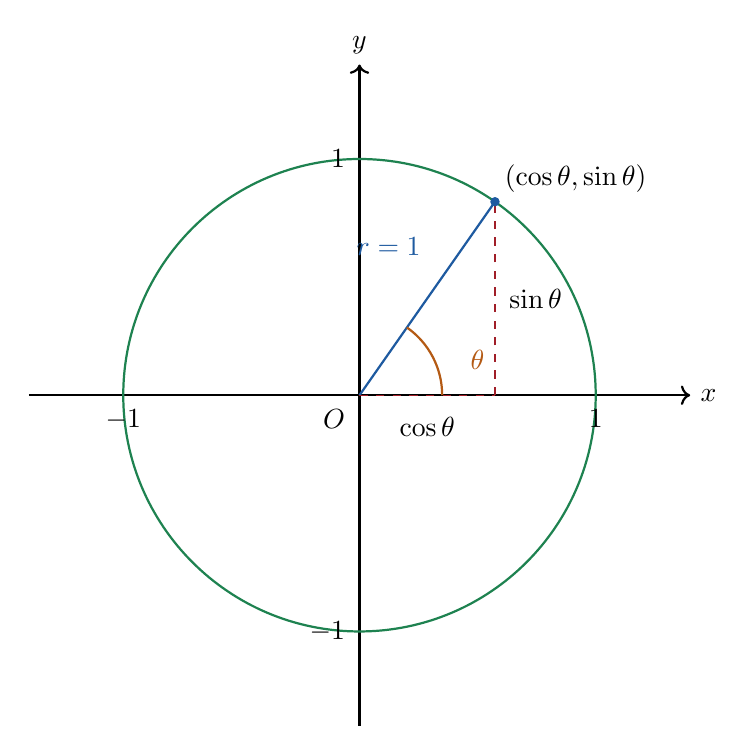
\begin{tikzpicture}[scale=3]
  % Axes
  \draw[->, thick] (-1.4, 0) -- (1.4, 0) node[right] {$x$};
  \draw[->, thick] (0, -1.4) -- (0, 1.4) node[above] {$y$};
  % Circle
  \draw[thick, sectiongreen] (0,0) circle (1);
  % Angle
  \draw[thick, sectionblue] (0,0) -- (55:1);
  \draw[dashed, sectionred] ({cos(55)}, 0) -- ({cos(55)}, {sin(55)});
  \draw[dashed, sectionred] (0, 0) -- ({cos(55)}, 0);
  % Angle arc
  \draw[thick, sectionorange] (0.35, 0) arc (0:55:0.35);
  \node[sectionorange] at (0.5, 0.15) {$\theta$};
  % Point
  \fill[sectionblue] ({cos(55)}, {sin(55)}) circle (0.02);
  \node[above right] at ({cos(55)}, {sin(55)}) {$(\cos\theta, \sin\theta)$};
  % Labels
  \node[below] at ({cos(55)/2}, -0.05) {$\cos\theta$};
  \node[right] at ({cos(55) + 0.02}, {sin(55)/2}) {$\sin\theta$};
  \node[above left, sectionblue] at (0.3, 0.55) {$r = 1$};
  % Axis labels
  \node[below left] at (-0.02, -0.02) {$O$};
  \node[below] at (1, -0.02) {$1$};
  \node[left] at (-0.02, 1) {$1$};
  \node[below] at (-1, -0.02) {$-1$};
  \node[left] at (-0.02, -1) {$-1$};
\end{tikzpicture}
\end{center}

\reftopic{Special Angles Table}

The angles $0^\circ, 30^\circ, 45^\circ, 60^\circ, 90^\circ$ correspond to points on the unit circle you must know cold.

\noindent
{\renewcommand{\arraystretch}{1.8}
\begin{tabularx}{\textwidth}{>{\centering\arraybackslash}p{2cm}
                              >{\centering\arraybackslash}p{2cm}
                              >{\centering\arraybackslash}X
                              >{\centering\arraybackslash}X
                              >{\centering\arraybackslash}X}
\toprule
\rowcolor{tableheadergreen}
\textbf{Angle} & \textbf{Radians} & \textbf{$\cos\theta$ ($x$)} & \textbf{$\sin\theta$ ($y$)} & \textbf{$\tan\theta$ ($y/x$)} \\
\midrule
\rowcolor{rowBg} $0^\circ$    & $0$              & $1$                        & $0$                        & $0$ \\
\rowcolor{rowA}  $30^\circ$   & $\pi/6$          & $\dfrac{\sqrt{3}}{2}$      & $\dfrac{1}{2}$             & $\dfrac{1}{\sqrt{3}} = \dfrac{\sqrt{3}}{3}$ \\
\rowcolor{rowBg} $45^\circ$   & $\pi/4$          & $\dfrac{\sqrt{2}}{2}$      & $\dfrac{\sqrt{2}}{2}$      & $1$ \\
\rowcolor{rowA}  $60^\circ$   & $\pi/3$          & $\dfrac{1}{2}$             & $\dfrac{\sqrt{3}}{2}$      & $\sqrt{3}$ \\
\rowcolor{rowBg} $90^\circ$   & $\pi/2$          & $0$                        & $1$                        & \textbf{undefined} \\
\bottomrule
\end{tabularx}}

\reftopic{The Sine Memory Trick}

Instead of memorizing five separate fractions, notice the pattern in sine values:
\[
  \sin(0^\circ),\; \sin(30^\circ),\; \sin(45^\circ),\; \sin(60^\circ),\; \sin(90^\circ)
  \;=\;
  \frac{\sqrt{0}}{2},\; \frac{\sqrt{1}}{2},\; \frac{\sqrt{2}}{2},\; \frac{\sqrt{3}}{2},\; \frac{\sqrt{4}}{2}
\]
which simplifies to
\[
  0,\quad \frac{1}{2},\quad \frac{\sqrt{2}}{2},\quad \frac{\sqrt{3}}{2},\quad 1
\]
\textbf{Cosine is the exact same sequence reversed.} That's the entire table --- one pattern, read forward for sine, backward for cosine.

\newpage

\reftopic{Graphs of Sine, Cosine \& Tangent}

To graph the trig functions, unroll the unit circle along a horizontal $\theta$-axis. As $\theta$ increases, the $y$-coordinate traces out $\sin\theta$; the $x$-coordinate traces out $\cos\theta$.

\subsection*{$y = \sin(x)$}

\begin{center}
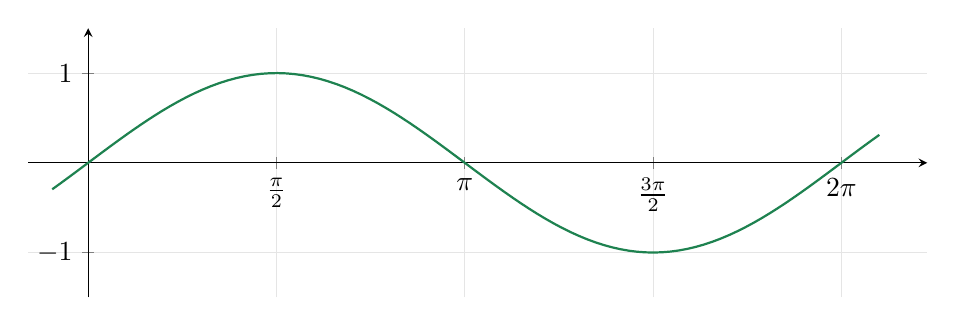
\begin{tikzpicture}
\begin{axis}[
  width=13cm, height=5cm,
  xmin=-0.5, xmax=7,
  ymin=-1.5, ymax=1.5,
  xtick={0, 1.5708, 3.1416, 4.7124, 6.2832},
  xticklabels={$0$, $\frac{\pi}{2}$, $\pi$, $\frac{3\pi}{2}$, $2\pi$},
  ytick={-1, 0, 1},
  axis lines=middle,
  grid=major, grid style={gray!20},
  samples=100, domain=-0.3:6.6,
]
\addplot[thick, sectiongreen] {sin(deg(x))};
\end{axis}
\end{tikzpicture}
\end{center}

\textbf{Sine wave:} starts at $0$, peaks at $1$ when $\theta = 90^\circ$, drops to $0$ at $180^\circ$, hits $-1$ at $270^\circ$, back to $0$ at $360^\circ$. Period $= 2\pi$; amplitude $= 1$.

\subsection*{$y = \cos(x)$}

\begin{center}
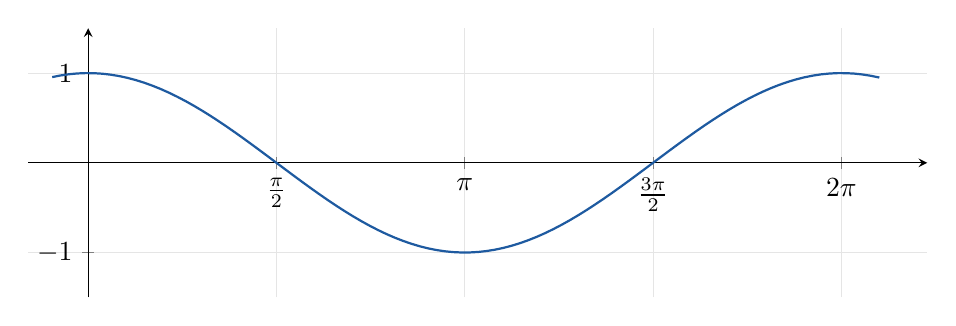
\begin{tikzpicture}
\begin{axis}[
  width=13cm, height=5cm,
  xmin=-0.5, xmax=7,
  ymin=-1.5, ymax=1.5,
  xtick={0, 1.5708, 3.1416, 4.7124, 6.2832},
  xticklabels={$0$, $\frac{\pi}{2}$, $\pi$, $\frac{3\pi}{2}$, $2\pi$},
  ytick={-1, 0, 1},
  axis lines=middle,
  grid=major, grid style={gray!20},
  samples=100, domain=-0.3:6.6,
]
\addplot[thick, sectionblue] {cos(deg(x))};
\end{axis}
\end{tikzpicture}
\end{center}

\textbf{Cosine wave:} starts at $1$, drops to $0$ at $90^\circ$, hits $-1$ at $180^\circ$, back to $0$ at $270^\circ$, back to $1$ at $360^\circ$. It's the sine wave shifted left by $\frac{\pi}{2}$ ($90^\circ$).

\subsection*{$y = \tan(x)$}

\begin{center}
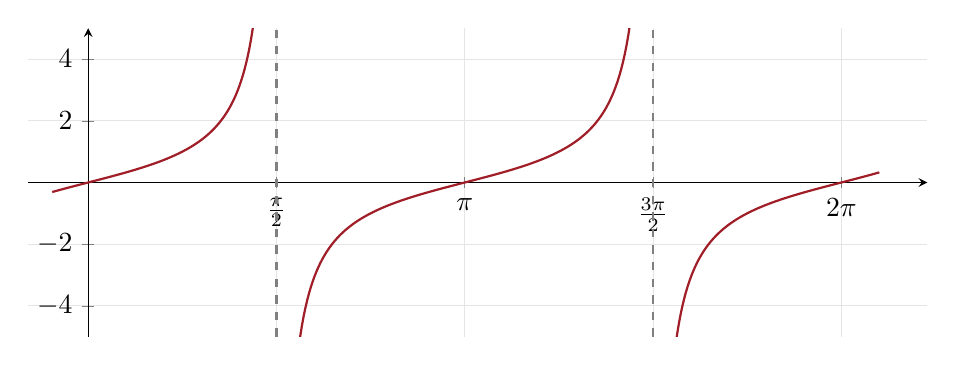
\begin{tikzpicture}
\begin{axis}[
  width=13cm, height=5.5cm,
  xmin=-0.5, xmax=7,
  ymin=-5, ymax=5,
  xtick={0, 1.5708, 3.1416, 4.7124, 6.2832},
  xticklabels={$0$, $\frac{\pi}{2}$, $\pi$, $\frac{3\pi}{2}$, $2\pi$},
  ytick={-4, -2, 0, 2, 4},
  axis lines=middle,
  grid=major, grid style={gray!20},
  samples=200,
]
\addplot[thick, sectionred, domain=-0.3:1.51] {tan(deg(x))};
\addplot[thick, sectionred, domain=1.63:4.66] {tan(deg(x))};
\addplot[thick, sectionred, domain=4.77:6.6] {tan(deg(x))};
\addplot[dashed, gray, thick] coordinates {(1.5708, -5) (1.5708, 5)};
\addplot[dashed, gray, thick] coordinates {(4.7124, -5) (4.7124, 5)};
\end{axis}
\end{tikzpicture}
\end{center}

\textbf{Tangent:} defined as $\sin(x)/\cos(x)$. Shoots to $+\infty$ as $x$ approaches $\frac{\pi}{2}$ (because $\cos(x) \to 0$). Has a \textbf{vertical asymptote} at every $\frac{\pi}{2} + n\pi$. Period $= \pi$ (repeats every $180^\circ$, not $360^\circ$ like sine and cosine).

\newpage

%% =============================================================================
%%  PART V -- Functions: Domain, Range & Restrictions
%% =============================================================================
\orangesections
\phantomsection
\addcontentsline{toc}{section}{\textcolor{sectionorange}{PART V \textemdash\ Functions: Domain, Range \& Restrictions}}
\partbanner{part4bg}{sectionorange}{Part V \quad Functions: Domain, Range \& Restrictions}

\vspace{6pt}

\reftopic{Domain \& Range from a Graph}

Every function has two questions to answer:

\begin{itemize}[noitemsep]
  \item \textbf{Domain} = all \emph{valid inputs} ($x$-values) the function accepts.
  \item \textbf{Range}  = all \emph{possible outputs} ($y$-values) the function produces.
\end{itemize}

\noindent
{\renewcommand{\arraystretch}{1.6}
\begin{tabularx}{\textwidth}{>{\bfseries\raggedright\arraybackslash}p{2.5cm}
                              >{\raggedright\arraybackslash}X
                              >{\raggedright\arraybackslash}X}
\toprule
\rowcolor{tableheaderorange}
\textbf{Concept} & \textbf{What to look for} & \textbf{For $f(x) = \sqrt{x-3}$} \\
\midrule
\rowcolor{rowOr} Domain & Look \textbf{left-to-right} on the graph. Where does it exist? Any gaps, holes, or asymptotes? & Starts at $x = 3$, extends right forever. \newline \textbf{Domain:} $[3, \infty)$ or $x \geq 3$ \\
\rowcolor{rowA}  Range  & Look \textbf{bottom-to-top}. What is the lowest and highest $y$-value? & Lowest $y = 0$ at $x=3$, rises forever. \newline \textbf{Range:} $[0, \infty)$ or $y \geq 0$ \\
\bottomrule
\end{tabularx}}

\begin{center}
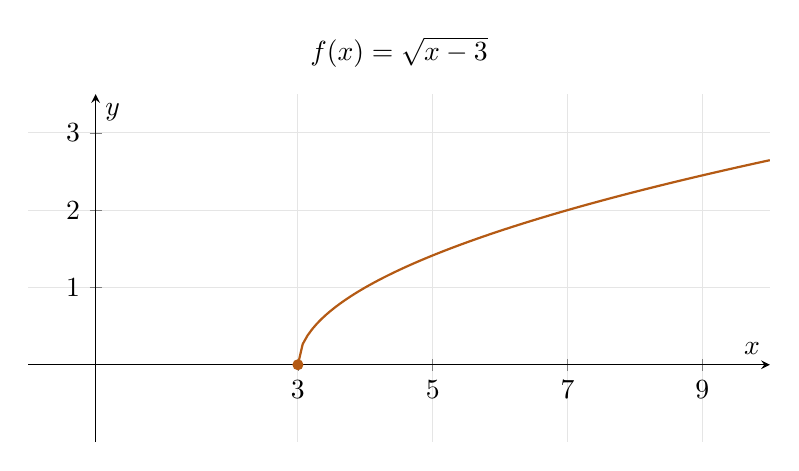
\begin{tikzpicture}
\begin{axis}[
  width=11cm, height=6cm,
  xmin=-1, xmax=10,
  ymin=-1, ymax=3.5,
  xtick={0, 3, 5, 7, 9},
  ytick={0, 1, 2, 3},
  axis lines=middle,
  xlabel=$x$, ylabel=$y$,
  grid=major, grid style={gray!20},
  samples=100, domain=3:10,
  title={$f(x) = \sqrt{x-3}$},
]
\addplot[thick, sectionorange] {sqrt(x-3)};
\fill[sectionorange] (axis cs:3, 0) circle (2pt);
\end{axis}
\end{tikzpicture}
\end{center}

\reftopic{Domain Restriction Red Flags}

Certain expressions have inputs that break math. Learn to spot these instantly.

\noindent
{\renewcommand{\arraystretch}{1.6}
\begin{tabularx}{\textwidth}{>{\bfseries\raggedright\arraybackslash}p{3.5cm}
                              >{\raggedright\arraybackslash}p{3.5cm}
                              >{\raggedright\arraybackslash}X}
\toprule
\rowcolor{tableheaderorange}
\textbf{Red Flag} & \textbf{Why It Fails} & \textbf{What to Look Out For} \\
\midrule
\rowcolor{rowOr} Division by Zero \newline ($\frac{\text{something}}{0}$) & Undefined & \textbf{Holes} (if factor cancels) or \textbf{Vertical Asymptotes} (if factor doesn't cancel). \\
\rowcolor{rowA}  Even Root of Negative \newline ($\sqrt{-x}$) & No real solution & Creates domain boundaries: $f(x) = \sqrt{x - 3}$ requires $x \geq 3$. Gives complex/imaginary output. \\
\rowcolor{rowOr} Logarithm of $\leq 0$ \newline ($\ln(x)$) & Undefined & Requires $x > 0$. Creates a vertical asymptote at $x = 0$. \\
\rowcolor{rowA}  Extraneous Solutions & Algebraic artifact & Happens when you square both sides or multiply by a variable expression. Always plug answers back into the \emph{original} equation to verify. \\
\bottomrule
\end{tabularx}}

\begin{tcolorbox}[colback=part4bg, colframe=sectionorange, arc=3pt, boxrule=1pt]
\textbf{Does $\sqrt{x-3}$ always give imaginary output?} \textbf{No.} It's only imaginary if $x < 3$ (because $x-3$ is negative). As long as $x \geq 3$, the output is a perfectly real number:
\begin{itemize}[noitemsep, leftmargin=*]
  \item $x = 3$: $\sqrt{0} = 0$
  \item $x = 4$: $\sqrt{1} = 1$
  \item $x = 7$: $\sqrt{4} = 2$
\end{itemize}
\end{tcolorbox}

\newpage

%% =============================================================================
%%  PART VI -- Rational Functions: Holes vs Asymptotes
%% =============================================================================
\tealsections
\phantomsection
\addcontentsline{toc}{section}{\textcolor{sectionteal}{PART VI \textemdash\ Rational Functions: Holes vs Asymptotes}}
\partbanner{part5bg}{sectionteal}{Part VI \quad Rational Functions: Holes vs Asymptotes}

\vspace{6pt}

\reftopic{Rational Functions}

A \textbf{rational function} is a fraction with variables in the denominator:
\[
  f(x) = \frac{P(x)}{Q(x)}
\]
Both \textbf{holes} and \textbf{vertical asymptotes} occur where the \textbf{denominator equals zero}. The difference is whether the offending factor cancels with something in the numerator.

\noindent
{\renewcommand{\arraystretch}{1.6}
\begin{tabularx}{\textwidth}{>{\bfseries\raggedright\arraybackslash}p{4cm}
                              >{\raggedright\arraybackslash}X}
\toprule
\rowcolor{tableheaderteal}
\textbf{Feature} & \textbf{When it happens} \\
\midrule
\rowcolor{rowTe} Hole (removable discontinuity) & The zero-producing factor \textbf{cancels} with a matching factor in the numerator. \\
\rowcolor{rowA}  Vertical Asymptote & The zero-producing factor \textbf{does NOT cancel}. \\
\bottomrule
\end{tabularx}}

\reftopic{Holes (Removable Discontinuities)}

\example{
Consider $f(x) = \dfrac{x^2 - 4}{x - 2}$.\\[4pt]
Factor the numerator:
\[
f(x) = \frac{(x - 2)(x + 2)}{x - 2}
\]
The $(x - 2)$ factors \textbf{cancel}, leaving $y = x + 2$ --- but only for $x \neq 2$.\\[4pt]
\textbf{Find the hole:} set the canceled factor to zero: $x - 2 = 0 \implies x = 2$.\\
\textbf{Find the $y$-value:} plug $x = 2$ into the reduced expression: $2 + 2 = 4$.\\[4pt]
\textbf{Hole at $(2, 4)$.}
}

\reftopic{Vertical Asymptotes}

\example{
Consider $f(x) = \dfrac{1}{x - 2}$.\\[4pt]
The factor $(x - 2)$ is in the denominator and does not cancel with anything.\\[4pt]
Setting $x - 2 = 0 \implies$ \textbf{vertical asymptote at $x = 2$}. The graph shoots off to $+\infty$ from one side and $-\infty$ from the other.
}

\begin{center}
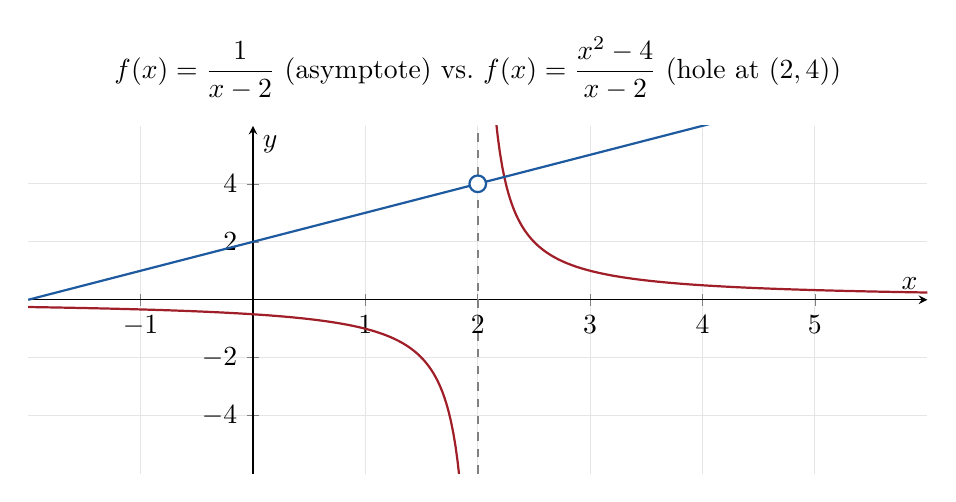
\begin{tikzpicture}
\begin{axis}[
  width=13cm, height=6cm,
  xmin=-2, xmax=6,
  ymin=-6, ymax=6,
  xtick={-1, 0, 1, 2, 3, 4, 5},
  ytick={-4, -2, 0, 2, 4},
  axis lines=middle,
  xlabel=$x$, ylabel=$y$,
  grid=major, grid style={gray!20},
  samples=200,
  title={$f(x) = \dfrac{1}{x-2}$ (asymptote) vs.\ $f(x) = \dfrac{x^2-4}{x-2}$ (hole at $(2, 4)$)},
]
\addplot[thick, sectionred, domain=-2:1.9] {1/(x-2)};
\addplot[thick, sectionred, domain=2.1:6] {1/(x-2)};
\addplot[dashed, gray, thick] coordinates {(2, -6) (2, 6)};
\addplot[thick, sectionblue, domain=-2:6] {x+2};
\draw[sectionblue, thick, fill=white] (axis cs:2, 4) circle (3pt);
\end{axis}
\end{tikzpicture}
\end{center}

\newpage

%% =============================================================================
%%  PART VII -- Introduction to Limits
%% =============================================================================
\redsections
\phantomsection
\addcontentsline{toc}{section}{\textcolor{sectionred}{PART VII \textemdash\ Introduction to Limits}}
\partbanner{part6bg}{sectionred}{Part VII \quad Introduction to Limits}

\vspace{6pt}

\reftopic{What is a Limit?}

The \textbf{limit} of a function $f(x)$ as $x$ approaches some value $a$ is the value $f(x)$ gets \emph{arbitrarily close to} --- not what $f(x)$ actually equals at $a$.

\[
  \lim_{x \to a} f(x) = L
\]
means ``as $x$ gets closer and closer to $a$, $f(x)$ gets closer and closer to $L$.''

\textbf{Why it matters:} limits let you talk about behavior at points where a function isn't defined (like holes) or at infinity. They are the foundation for both \textbf{derivatives} and \textbf{integrals} in calculus.

\subsection*{Direct Substitution}

If $f(x)$ is continuous at $a$ (no holes, no asymptotes, no domain issues), the limit is just $f(a)$:
\[
  \lim_{x \to 5} (x^2 + 1) = 5^2 + 1 = 26
\]
Always try direct substitution first. If it gives you a definite number, you're done.

\reftopic{One-Sided Limits}

Sometimes the limit depends on which side you approach from:

\noindent
{\renewcommand{\arraystretch}{1.6}
\begin{tabularx}{\textwidth}{>{\centering\arraybackslash}p{3cm}
                              >{\bfseries\raggedright\arraybackslash}p{4cm}
                              >{\raggedright\arraybackslash}X}
\toprule
\rowcolor{tableheaderred}
\textbf{Notation} & \textbf{Name} & \textbf{Meaning} \\
\midrule
\rowcolor{rowRe} $\lim_{x \to a^-} f(x)$ & Left-hand limit & Approach $a$ from values \emph{less than} $a$. \\
\rowcolor{rowA}  $\lim_{x \to a^+} f(x)$ & Right-hand limit & Approach $a$ from values \emph{greater than} $a$. \\
\bottomrule
\end{tabularx}}

\begin{tcolorbox}[colback=part6bg, colframe=sectionred, arc=3pt, boxrule=1pt]
\textbf{Existence rule:} The overall limit $\lim_{x \to a} f(x)$ exists \emph{if and only if} the left-hand and right-hand limits both exist \emph{and are equal}:
\[
  \lim_{x \to a} f(x) = L \iff \lim_{x \to a^-} f(x) = L = \lim_{x \to a^+} f(x)
\]
If they disagree, the limit \textbf{does not exist (DNE)}.
\end{tcolorbox}

\reftopic{When Limits Do Not Exist (DNE)}

A limit fails to exist for three main reasons:
\begin{enumerate}[noitemsep]
  \item \textbf{Jump discontinuity:} left-hand and right-hand limits are different values.
  \item \textbf{Infinite behavior:} function grows without bound (vertical asymptote).
  \item \textbf{Oscillation:} function oscillates infinitely often near the point (e.g., $\sin(1/x)$ near $x = 0$).
\end{enumerate}

Also, if the point isn't in the function's domain \emph{and} you can't approach it from both sides, the limit doesn't exist in the standard sense.

\reftopic{The Squeeze Theorem}

Also called the \textbf{Sandwich Theorem}. If you can trap a hard-to-evaluate function between two easier ones that share the same limit, the middle function must have that limit too.

\begin{tcolorbox}[colback=part6bg, colframe=sectionred, arc=3pt, boxrule=1pt]
If $g(x) \leq f(x) \leq h(x)$ for all $x$ near $a$, and
\[
  \lim_{x \to a} g(x) = \lim_{x \to a} h(x) = L
\]
then
\[
  \lim_{x \to a} f(x) = L.
\]
\end{tcolorbox}

\example{
\textbf{Given:} $4x - 9 \leq f(x) \leq x^2 - 4x + 7$ near $x = 4$. Find $\displaystyle \lim_{x \to 4} f(x)$.\\[4pt]
Evaluate the two bounding functions at $x = 4$:
\begin{itemize}[noitemsep, leftmargin=*]
  \item Lower: $g(4) = 4(4) - 9 = 16 - 9 = 7$
  \item Upper: $h(4) = 4^2 - 4(4) + 7 = 16 - 16 + 7 = 7$
\end{itemize}
Both bounds equal $7$ at $x = 4$. So $f(x)$ is squeezed between two functions that both approach $7$.
\[
  \lim_{x \to 4} f(x) = \boxed{7}
\]
}

\begin{center}
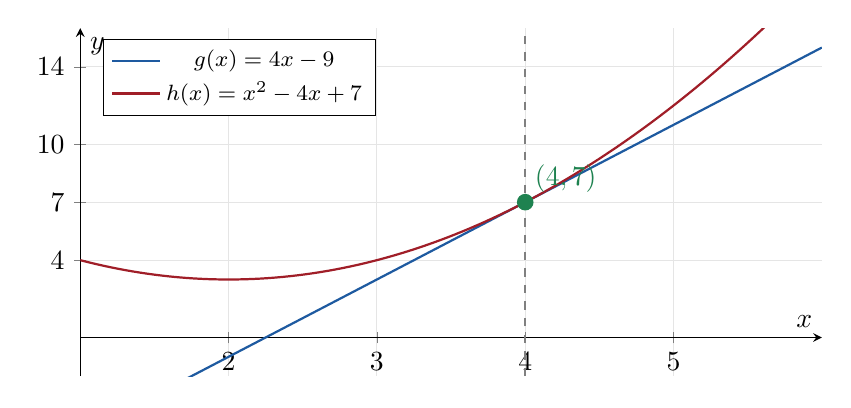
\begin{tikzpicture}
\begin{axis}[
  width=11cm, height=6cm,
  xmin=1, xmax=6,
  ymin=-2, ymax=16,
  xtick={2, 3, 4, 5},
  ytick={0, 4, 7, 10, 14},
  axis lines=middle,
  xlabel=$x$, ylabel=$y$,
  grid=major, grid style={gray!20},
  samples=100,
  legend pos=north west, legend style={font=\footnotesize},
]
\addplot[thick, sectionblue, domain=1:6] {4*x - 9};
\addlegendentry{$g(x) = 4x - 9$}
\addplot[thick, sectionred, domain=1:6] {x^2 - 4*x + 7};
\addlegendentry{$h(x) = x^2 - 4x + 7$}
\addplot[dashed, gray, thick] coordinates {(4, -2) (4, 16)};
\fill[sectiongreen] (axis cs:4, 7) circle (3pt);
\node[sectiongreen, above right] at (axis cs:4, 7) {$(4, 7)$};
\end{axis}
\end{tikzpicture}
\end{center}

Both curves meet at exactly $(4, 7)$ --- so whatever $f(x)$ is doing between them, it has no choice but to pass through $y = 7$ at $x = 4$.

\reftopic{Limits with Square Roots}

\example{
\textbf{Find $\displaystyle \lim_{x \to 5} \sqrt{x - 3}$:}\\[4pt]
Since $x = 5$ is well inside the domain ($5 \geq 3$), use direct substitution:
\[
  \lim_{x \to 5} \sqrt{x - 3} = \sqrt{5 - 3} = \sqrt{2} \approx 1.414
\]
}

\example{
\textbf{Find $\displaystyle \lim_{x \to 2} \sqrt{x - 3}$:}\\[4pt]
Here $x = 2$ lies \emph{outside} the function's domain ($x \geq 3$ is required). Neither one-sided limit is defined in the reals --- there's no way to approach $x = 2$ while staying in the domain.\\[4pt]
\textbf{Limit does not exist (DNE)} in real-valued calculus.
}


%% =============================================================================
%%  PART VIII -- Periodic Functions & Bounded Squeeze Problems
%% =============================================================================
\bluesections
\phantomsection
\addcontentsline{toc}{section}{\textcolor{sectionblue}{PART VIII \textemdash\ Periodic Functions \& Bounded Squeeze Problems}}
\partbanner{partbg}{sectionblue}{Part VIII \quad Periodic Functions \& Bounded Squeeze Problems}

\vspace{6pt}
\begin{center}\small\itshape
  Some functions oscillate wildly and have no ordinary limit --- but you can still tame them
  by squeezing them between two bounds. This is one of the most useful ideas in calculus.
\end{center}

\reftopic{What is a Periodic Function?}

A function $f(x)$ is \textbf{periodic} if it repeats itself over a fixed interval called the \textbf{period} $T$:
\[
  f(x + T) = f(x) \quad \text{for all } x
\]
The most famous examples are $\sin(x)$ and $\cos(x)$, both with period $T = 2\pi$. Tangent has period $\pi$.

\begin{tcolorbox}[colback=partbg, colframe=sectionblue, arc=3pt, boxrule=1pt]
\textbf{Two things every periodic function has:}
\begin{itemize}[noitemsep, leftmargin=*]
  \item A \textbf{period} $T$: how often the pattern repeats.
  \item An \textbf{amplitude}: the maximum distance from the center line.
\end{itemize}
For sine and cosine, amplitude $= 1$: they never go above $1$ or below $-1$.
\end{tcolorbox}

\reftopic{Bounded Trig Functions ($-1 \leq \sin, \cos \leq 1$)}

The critical fact about sine and cosine is that they are \textbf{always bounded}:
\[
  \boxed{\; -1 \leq \sin(\text{anything}) \leq 1 \qquad -1 \leq \cos(\text{anything}) \leq 1 \;}
\]

\textbf{The key word is ``anything''} --- the inside of the sine or cosine can be $x$, or $2x$, or $\frac{2}{x}$, or $\ln(x)$, or the most ridiculous expression you can imagine. \emph{The output is still trapped between $-1$ and $1$.} This is what makes them so useful in the Squeeze Theorem.

\example{
For any real $u$: $\; -1 \leq \cos(u) \leq 1$\\[2pt]
In particular, if $u = \frac{2}{x}$:
\[
  -1 \leq \cos\!\left(\frac{2}{x}\right) \leq 1 \quad \text{for all } x \neq 0
\]
Even though $\cos(2/x)$ oscillates infinitely fast near $x = 0$, its output is still trapped in $[-1, 1]$.
}

\reftopic{The Classic Problem: $\cos(1/x)$ as $x \to 0$}

Consider what $\cos(1/x)$ does near $x = 0$. As $x$ gets closer to zero, $1/x$ shoots off to $\infty$ --- which means $\cos(1/x)$ cycles through its full range $[-1, 1]$ an infinite number of times inside any tiny interval around $0$.

\begin{center}
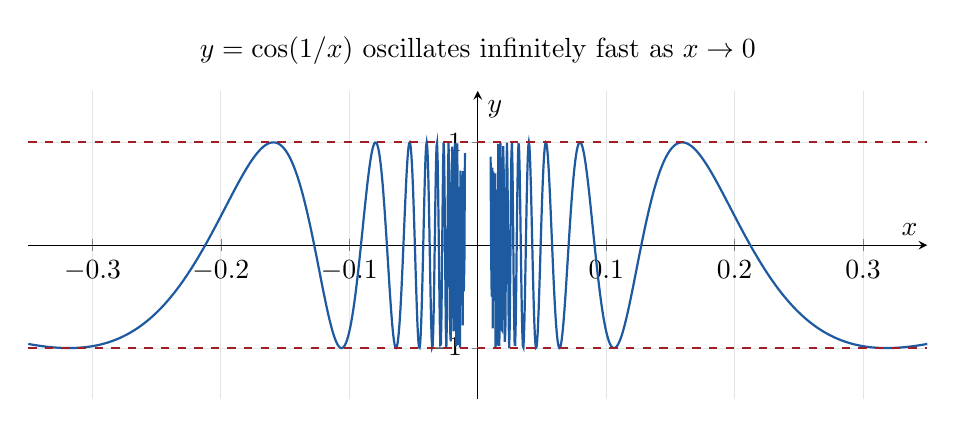
\begin{tikzpicture}
\begin{axis}[
  width=13cm, height=5.5cm,
  xmin=-0.35, xmax=0.35,
  ymin=-1.5, ymax=1.5,
  xtick={-0.3, -0.2, -0.1, 0, 0.1, 0.2, 0.3},
  ytick={-1, 0, 1},
  axis lines=middle,
  xlabel=$x$, ylabel=$y$,
  grid=major, grid style={gray!20},
  samples=800,
  title={$y = \cos(1/x)$ oscillates infinitely fast as $x \to 0$},
]
\addplot[thick, sectionblue, domain=-0.35:-0.01] {cos(deg(1/x))};
\addplot[thick, sectionblue, domain=0.01:0.35] {cos(deg(1/x))};
\addplot[dashed, sectionred, thick] coordinates {(-0.35, 1) (0.35, 1)};
\addplot[dashed, sectionred, thick] coordinates {(-0.35, -1) (0.35, -1)};
\end{axis}
\end{tikzpicture}
\end{center}

\begin{tcolorbox}[colback=partbg, colframe=sectionblue, arc=3pt, boxrule=1pt]
\textbf{Verdict:} $\displaystyle \lim_{x \to 0} \cos\!\left(\frac{1}{x}\right)$ \textbf{does not exist (DNE)}.\\[4pt]
The function doesn't approach any single value --- it oscillates infinitely between $-1$ and $1$. But this alone doesn't tell you what happens when $\cos(1/x)$ is multiplied by something else!
\end{tcolorbox}

\reftopic{Squeezing with a Multiplier: $x^2\cos(1/x)$}

Now for the interesting case. Consider:
\[
  \lim_{x \to 0} x^2 \cos\!\left(\frac{1}{x}\right)
\]

The $\cos(1/x)$ part still oscillates wildly. But we're now multiplying it by $x^2$, which is going to zero. Which wins?

\textbf{Set up the squeeze:} We know that for all $x \neq 0$:
\[
  -1 \leq \cos\!\left(\frac{1}{x}\right) \leq 1
\]
Multiply everything by $x^2$. Because $x^2 \geq 0$ (it never flips inequalities), we get:
\[
  -x^2 \leq x^2 \cos\!\left(\frac{1}{x}\right) \leq x^2
\]

\textbf{Take limits of the outer bounds:}
\[
  \lim_{x \to 0} (-x^2) = 0 \qquad \lim_{x \to 0} (x^2) = 0
\]

Both bounds go to $0$. By the Squeeze Theorem, the middle is squeezed to $0$ as well:
\[
  \boxed{\; \lim_{x \to 0} x^2 \cos\!\left(\frac{1}{x}\right) = 0 \;}
\]

\begin{center}
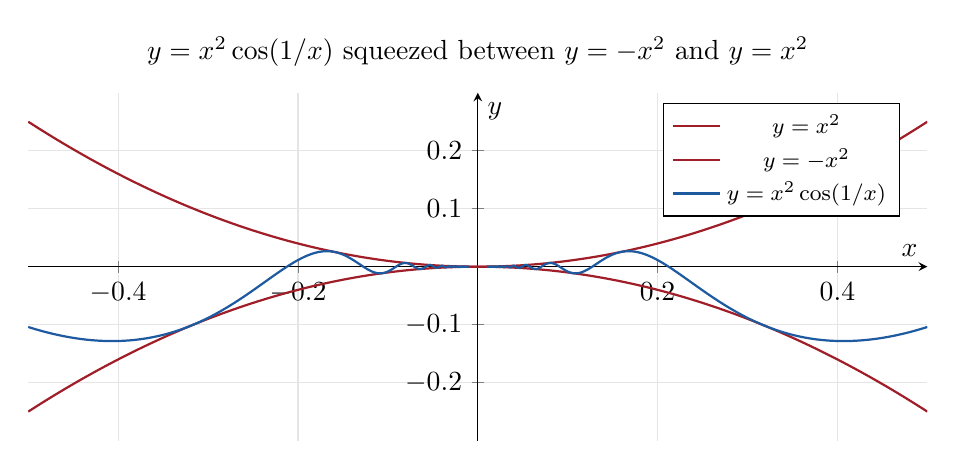
\begin{tikzpicture}
\begin{axis}[
  width=13cm, height=6cm,
  xmin=-0.5, xmax=0.5,
  ymin=-0.3, ymax=0.3,
  xtick={-0.4, -0.2, 0, 0.2, 0.4},
  ytick={-0.2, -0.1, 0, 0.1, 0.2},
  axis lines=middle,
  xlabel=$x$, ylabel=$y$,
  grid=major, grid style={gray!20},
  samples=800,
  legend pos=north east, legend style={font=\footnotesize},
  title={$y = x^2\cos(1/x)$ squeezed between $y = -x^2$ and $y = x^2$},
]
\addplot[thick, sectionred, domain=-0.5:0.5] {x^2};
\addlegendentry{$y = x^2$}
\addplot[thick, sectionred, domain=-0.5:0.5] {-x^2};
\addlegendentry{$y = -x^2$}
\addplot[thick, sectionblue, domain=-0.5:-0.01] {x^2 * cos(deg(1/x))};
\addplot[thick, sectionblue, domain=0.01:0.5, forget plot] {x^2 * cos(deg(1/x))};
\addlegendentry{$y = x^2\cos(1/x)$}
\end{axis}
\end{tikzpicture}
\end{center}

\textbf{Reading the graph:} The two red parabolas ($y = \pm x^2$) form a ``funnel'' that pinches to zero at $x = 0$. No matter how much the blue oscillating curve wiggles, it's forced into that funnel --- and the funnel forces it to $0$.

\reftopic{When Bounded $\times$ Zero Wins}

This pattern comes up constantly in limits. If you have a product where one factor is \textbf{bounded} and the other goes to \textbf{zero}, the whole product goes to zero.

\begin{tcolorbox}[colback=partbg, colframe=sectionblue,
  title={\bfseries The Bounded-Times-Zero Rule}, arc=3pt, boxrule=1pt]
If $|f(x)| \leq M$ for some constant $M$, and $\displaystyle \lim_{x \to a} g(x) = 0$, then
\[
  \lim_{x \to a} f(x) \cdot g(x) = 0
\]
No matter how ugly, oscillating, or discontinuous $f(x)$ is --- as long as it's \emph{bounded}, multiplying by something that goes to zero kills it.
\end{tcolorbox}

\subsection*{More Examples}

\example{
\textbf{Find $\displaystyle \lim_{x \to 0} x \sin\!\left(\frac{1}{x}\right)$.}\\[4pt]
$\sin(1/x)$ is bounded: $-1 \leq \sin(1/x) \leq 1$. So
\[
  -|x| \leq x \sin\!\left(\frac{1}{x}\right) \leq |x|
\]
Both $\pm|x| \to 0$ as $x \to 0$. By Squeeze: $\displaystyle \lim_{x \to 0} x \sin\!\left(\frac{1}{x}\right) = 0$.
}

\example{
\textbf{Find $\displaystyle \lim_{x \to 0} x^3 \cos\!\left(\frac{5}{x^2}\right)$.}\\[4pt]
$\cos(5/x^2)$ is bounded: $-1 \leq \cos(5/x^2) \leq 1$. Multiply by $x^3$ (careful, this can be negative). Use absolute values:
\[
  \left| x^3 \cos\!\left(\frac{5}{x^2}\right) \right| \leq |x^3|
\]
Since $|x^3| \to 0$ as $x \to 0$, by squeeze the limit is $\boxed{0}$.
}

\example{
\textbf{Find $\displaystyle \lim_{x \to \infty} \frac{\sin(x)}{x}$.}\\[4pt]
$\sin(x)$ is bounded: $-1 \leq \sin(x) \leq 1$. Divide by $x$ (positive as $x \to \infty$):
\[
  -\frac{1}{x} \leq \frac{\sin(x)}{x} \leq \frac{1}{x}
\]
Both $\pm 1/x \to 0$. Squeeze gives $\displaystyle \lim_{x \to \infty} \frac{\sin(x)}{x} = 0$.
\\[3pt]
\textit{Note: this is different from the famous $\lim_{x \to 0} \frac{\sin x}{x} = 1$ --- that's a distinct classic limit worth memorizing separately.}
}

\subsection*{When the Rule Does NOT Apply}

\warning{
The bounded-times-zero rule requires that the \emph{other} factor genuinely goes to zero. If you have an oscillating function multiplied by a constant or by something bounded away from zero, the limit still doesn't exist.
\\[4pt]
For example: $\displaystyle \lim_{x \to 0} \cos\!\left(\frac{1}{x}\right)$ still DNE --- there's no factor going to zero to kill the oscillation. And $\displaystyle \lim_{x \to 0} 5 \cos\!\left(\frac{1}{x}\right)$ also DNE for the same reason.
}

\newpage

%% =============================================================================
%%  PART IX -- Exponentials, Logarithms & Euler's Number
%% =============================================================================
\greysections
\phantomsection
\addcontentsline{toc}{section}{\textcolor{sectiongrey}{PART IX \textemdash\ Exponentials, Logarithms \& Euler's Number}}
\partbanner{part7bg}{sectiongrey}{Part IX \quad Exponentials, Logarithms \& Euler's Number}

\vspace{6pt}

\reftopic{What is $e$?}

$e$ (Euler's number) is a mathematical constant approximately equal to
\[
  e \approx 2.71828\ldots
\]

It is the \textbf{continuous growth constant}. It naturally appears anywhere something grows or decays proportionally to its current size --- interest compounding every microsecond, populations growing, radioactive decay, heat cooling. Just like $\pi$ comes up wherever circles are involved, $e$ comes up wherever \emph{continuous} change is involved.

\textbf{One way to define $e$:} 
\[
  e = \lim_{n \to \infty} \left(1 + \frac{1}{n}\right)^n
\]
This is what you get if you take ``100\% growth'' and compound it infinitely often.

\reftopic{The Natural Logarithm $\ln$}

The logarithm with base $e$ is called the \textbf{natural logarithm}, written $\ln(x)$ instead of $\log_e(x)$.

\begin{tcolorbox}[colback=part7bg, colframe=sectiongrey, arc=3pt, boxrule=1pt]
\textbf{Think of it like a growth engine and a stopwatch:}
\begin{itemize}[noitemsep, leftmargin=*]
  \item $e^x$ is the \textbf{growth engine}: you give it a time/rate $x$, it returns the final amount.
  \item $\ln(x)$ is the \textbf{time finder}: you give it a target amount $x$, it returns how much time was needed to grow that much.
\end{itemize}
Because they are exact inverses of each other:
\[
  \ln(e^x) = x \qquad\text{and}\qquad e^{\ln(x)} = x
\]
\end{tcolorbox}

\reftopic{Continuous Growth \& Decay}

Instead of step-by-step (yearly, monthly) growth, real-world systems often grow continuously. The formula:
\[
  \boxed{\; A = P e^{rt} \;}
\]
where $P$ = starting principal, $r$ = growth rate (as decimal), $t$ = time, $A$ = final amount.

\example{
\textbf{Doubling Time Problem:} How long does it take for an investment to double at $5\%$ continuous interest?\\[4pt]
Set $A = 2P$ (doubled) and solve for $t$:
\[
  2P = P e^{0.05 t} \implies e^{0.05 t} = 2
\]
Take the natural log of both sides:
\[
  \ln(e^{0.05 t}) = \ln(2) \implies 0.05 t = \ln(2)
\]
\[
  t = \frac{\ln(2)}{0.05} \approx \frac{0.693}{0.05} \approx 13.86 \text{ years}
\]
\textit{This is where the ``Rule of 72'' comes from --- $72 / 5 \approx 14.4$ years is a close approximation for annual compounding.}
}

\reftopic{Calculus Properties of $e^x$ and $\ln(x)$}

The reason $e$ shows up everywhere in calculus is these two beautiful properties:

\begin{tcolorbox}[colback=part7bg, colframe=sectiongrey, arc=3pt, boxrule=1pt]
\textbf{$e^x$ is its own derivative:}
\[
  \frac{d}{dx}(e^x) = e^x
\]
The rate at which $e^x$ grows at any exact moment \emph{equals its current value}. Every constant multiple $Ce^x$ has this property too. $e^x$ is the mathematical embodiment of ``the more you have, the faster you grow.''\\[6pt]
\textbf{$\ln(x)$ solves an integration gap:}
\[
  \int \frac{1}{x}\, dx = \ln|x| + C
\]
The power rule $\int x^n\, dx = \frac{x^{n+1}}{n+1}$ breaks down when $n = -1$ (division by zero). $\ln|x|$ fills that gap.
\end{tcolorbox}

\reftopic{Change of Base Formula}

Natural log is the standard log in scientific computing (in most programming languages, \texttt{log()} defaults to $\ln$). Any other logarithm can be converted using:
\[
  \boxed{\; \log_b(a) = \frac{\ln(a)}{\ln(b)} \;}
\]

\example{
\textbf{Compute $\log_2(8)$ using natural logs:}
\[
  \log_2(8) = \frac{\ln(8)}{\ln(2)} = \frac{2.0794}{0.6931} = 3
\]
(Which checks: $2^3 = 8$.)
}

%% =============================================================================
%%  PART X -- Advanced Formulas & Identities
%% =============================================================================
\greensections
\phantomsection
\addcontentsline{toc}{section}{\textcolor{sectiongreen}{PART X \textemdash\ Connected Formula Toolkit}}
\partbanner{part2bg}{sectiongreen}{Part X \quad Connected Formula Toolkit}

\vspace{6pt}
\begin{center}\small\itshape
  Use this as a connected roadmap: algebra simplifies expressions; trigonometric identities rewrite them;
  limits explain derivatives; derivative families lead directly to matching integrals.
\end{center}

\reftopic{Algebra Identities}

\noindent
{\renewcommand{\arraystretch}{1.7}
\begin{tabularx}{\textwidth}{>{\bfseries\raggedright\arraybackslash}p{4.5cm}
                              >{\raggedright\arraybackslash}X}
\toprule
\rowcolor{tableheadergreen}
\textbf{Identity} & \textbf{Formula} \\
\midrule
\rowcolor{rowBg} Difference of squares      & $a^2 - b^2 = (a-b)(a+b)$ \\
\rowcolor{rowA}  Sum of cubes               & $a^3 + b^3 = (a+b)(a^2 - ab + b^2)$ \\
\rowcolor{rowBg} Difference of cubes        & $a^3 - b^3 = (a-b)(a^2 + ab + b^2)$ \\
\rowcolor{rowA}  Perfect square (sum)       & $(a+b)^2 = a^2 + 2ab + b^2$ \\
\rowcolor{rowBg} Perfect square (difference)& $(a-b)^2 = a^2 - 2ab + b^2$ \\
\rowcolor{rowA}  Perfect cube (sum)         & $(a+b)^3 = a^3 + 3a^2 b + 3ab^2 + b^3$ \\
\rowcolor{rowBg} Binomial theorem           & $(a+b)^n = \sum_{k=0}^{n} \binom{n}{k} a^{n-k} b^k$ \\
\rowcolor{rowA}  Binomial coefficient       & $\binom{n}{k} = \dfrac{n!}{k!(n-k)!}$ \\
\rowcolor{rowBg} Quadratic formula          & $x = \dfrac{-b \pm \sqrt{b^2 - 4ac}}{2a}$ \\
\rowcolor{rowA}  Vertex of parabola $y = ax^2 + bx + c$ & $x_{\text{vertex}} = -\dfrac{b}{2a}$ \\
\rowcolor{rowBg} Distance formula           & $d = \sqrt{(x_2-x_1)^2 + (y_2-y_1)^2}$ \\
\rowcolor{rowA}  Midpoint formula           & $\left(\dfrac{x_1+x_2}{2}, \dfrac{y_1+y_2}{2}\right)$ \\
\rowcolor{rowBg} Slope of a line            & $m = \dfrac{y_2 - y_1}{x_2 - x_1}$ \\
\rowcolor{rowA}  Point-slope form           & $y - y_1 = m(x - x_1)$ \\
\bottomrule
\end{tabularx}}

\reftopic{Exponent \& Logarithm Rules}

\noindent
{\renewcommand{\arraystretch}{1.7}
\begin{tabularx}{\textwidth}{>{\bfseries\raggedright\arraybackslash}p{4cm}
                              >{\raggedright\arraybackslash}X}
\toprule
\rowcolor{tableheadergreen}
\textbf{Exponent Rule} & \textbf{Formula} \\
\midrule
\rowcolor{rowBg} Product of powers      & $x^a \cdot x^b = x^{a+b}$ \\
\rowcolor{rowA}  Quotient of powers     & $\dfrac{x^a}{x^b} = x^{a-b}$ \\
\rowcolor{rowBg} Power of a power       & $(x^a)^b = x^{ab}$ \\
\rowcolor{rowA}  Power of a product     & $(xy)^a = x^a y^a$ \\
\rowcolor{rowBg} Negative exponent      & $x^{-a} = \dfrac{1}{x^a}$ \\
\rowcolor{rowA}  Zero exponent          & $x^0 = 1$ \quad (for $x \neq 0$) \\
\rowcolor{rowBg} Fractional exponent    & $x^{a/b} = \sqrt[b]{x^a}$ \\
\bottomrule
\end{tabularx}}

\vspace{6pt}

\noindent
{\renewcommand{\arraystretch}{1.7}
\begin{tabularx}{\textwidth}{>{\bfseries\raggedright\arraybackslash}p{4cm}
                              >{\raggedright\arraybackslash}X}
\toprule
\rowcolor{tableheadergreen}
\textbf{Logarithm Rule} & \textbf{Formula} \\
\midrule
\rowcolor{rowBg} Product rule           & $\log_b(xy) = \log_b(x) + \log_b(y)$ \\
\rowcolor{rowA}  Quotient rule          & $\log_b\!\left(\dfrac{x}{y}\right) = \log_b(x) - \log_b(y)$ \\
\rowcolor{rowBg} Power rule             & $\log_b(x^n) = n \log_b(x)$ \\
\rowcolor{rowA}  Change of base         & $\log_b(x) = \dfrac{\ln(x)}{\ln(b)} = \dfrac{\log_{10}(x)}{\log_{10}(b)}$ \\
\rowcolor{rowBg} Inverse of exponential & $\log_b(b^x) = x$, \quad $b^{\log_b(x)} = x$ \\
\rowcolor{rowA}  Log of $1$             & $\log_b(1) = 0$ \\
\rowcolor{rowBg} Log of base            & $\log_b(b) = 1$ \\
\bottomrule
\end{tabularx}}

\reftopic{Trigonometric Identities}

\subsection*{Pythagorean Identities}

The three most important trig identities, all derived from $\sin^2 + \cos^2 = 1$:
\[
  \sin^2\theta + \cos^2\theta = 1
  \qquad
  1 + \tan^2\theta = \sec^2\theta
  \qquad
  1 + \cot^2\theta = \csc^2\theta
\]

\subsection*{Reciprocal Identities}

\[
  \csc\theta = \frac{1}{\sin\theta}
  \qquad
  \sec\theta = \frac{1}{\cos\theta}
  \qquad
  \cot\theta = \frac{1}{\tan\theta} = \frac{\cos\theta}{\sin\theta}
\]

\subsection*{Quotient Identity}

\[
  \tan\theta = \frac{\sin\theta}{\cos\theta}
\]

\subsection*{Even / Odd Identities}

\begin{center}
Even (symmetric across $y$-axis): $\quad \cos(-\theta) = \cos\theta \qquad \sec(-\theta) = \sec\theta$\\[3pt]
Odd (symmetric through origin): $\quad \sin(-\theta) = -\sin\theta \qquad \tan(-\theta) = -\tan\theta \qquad \csc(-\theta) = -\csc\theta$
\end{center}

\subsection*{Angle-Sum \& Difference Formulas}

\[
  \sin(a \pm b) = \sin a \cos b \pm \cos a \sin b
\]
\[
  \cos(a \pm b) = \cos a \cos b \mp \sin a \sin b
\]
\[
  \tan(a \pm b) = \frac{\tan a \pm \tan b}{1 \mp \tan a \tan b}
\]

\subsection*{Double-Angle Formulas}

\[
  \sin(2\theta) = 2 \sin\theta \cos\theta
\]
\[
  \cos(2\theta) = \cos^2\theta - \sin^2\theta = 2\cos^2\theta - 1 = 1 - 2\sin^2\theta
\]
\[
  \tan(2\theta) = \frac{2\tan\theta}{1 - \tan^2\theta}
\]

\subsection*{Half-Angle Formulas}

\[
  \sin^2\theta = \frac{1 - \cos(2\theta)}{2}
  \qquad
  \cos^2\theta = \frac{1 + \cos(2\theta)}{2}
\]

\reftopic{Trig Conversions, Angle Measures \& Inverses}

Every trig function can be written in terms of any other. These are the conversions you'll
reach for most often --- when simplifying, when rewriting integrals, or when a problem is
easier in one form than another.

\textbf{Reciprocal conversions (how to write any trig function in its reciprocal form):}

\noindent
{\small\renewcommand{\arraystretch}{1.7}
\begin{tabularx}{\textwidth}{>{\bfseries\raggedright\arraybackslash}p{3cm}
                              >{\raggedright\arraybackslash}X
                              >{\raggedright\arraybackslash}X}
\toprule
\rowcolor{tableheaderpurple}
\textbf{Function} & \textbf{Equals} & \textbf{Also equals} \\
\midrule
\rowcolor{rowPu} $\sin\theta$   & $\dfrac{1}{\csc\theta}$                    & $\cos\!\left(\tfrac{\pi}{2} - \theta\right)$ \\
\rowcolor{rowA}  $\cos\theta$   & $\dfrac{1}{\sec\theta}$                    & $\sin\!\left(\tfrac{\pi}{2} - \theta\right)$ \\
\rowcolor{rowPu} $\tan\theta$   & $\dfrac{1}{\cot\theta} = \dfrac{\sin\theta}{\cos\theta}$ & $\cot\!\left(\tfrac{\pi}{2} - \theta\right)$ \\
\rowcolor{rowA}  $\csc\theta$   & $\dfrac{1}{\sin\theta}$                    & $\sec\!\left(\tfrac{\pi}{2} - \theta\right)$ \\
\rowcolor{rowPu} $\sec\theta$   & $\dfrac{1}{\cos\theta}$                    & $\csc\!\left(\tfrac{\pi}{2} - \theta\right)$ \\
\rowcolor{rowA}  $\cot\theta$   & $\dfrac{1}{\tan\theta} = \dfrac{\cos\theta}{\sin\theta}$ & $\tan\!\left(\tfrac{\pi}{2} - \theta\right)$ \\
\bottomrule
\end{tabularx}}

\vspace{4pt}
\textit{Memory aid: the ``co-'' functions (\textbf{co}sine, \textbf{co}tangent, \textbf{co}secant) are the complementary partners of sine, tangent, and secant. Complementary = adds to $90^\circ$.}

\vspace{6pt}
\textbf{Squared conversions (rearrangements of the Pythagorean identities):}

\noindent
{\small\renewcommand{\arraystretch}{1.7}
\begin{tabularx}{\textwidth}{>{\bfseries\raggedright\arraybackslash}p{3cm}
                              >{\raggedright\arraybackslash}X}
\toprule
\rowcolor{tableheaderpurple}
\textbf{Squared Form} & \textbf{Equivalent Expression(s)} \\
\midrule
\rowcolor{rowPu} $\sin^2\theta$   & $1 - \cos^2\theta$ \quad or \quad $\dfrac{1 - \cos(2\theta)}{2}$ (half-angle form) \\
\rowcolor{rowA}  $\cos^2\theta$   & $1 - \sin^2\theta$ \quad or \quad $\dfrac{1 + \cos(2\theta)}{2}$ (half-angle form) \\
\rowcolor{rowPu} $\tan^2\theta$   & $\sec^2\theta - 1$ \quad or \quad $\dfrac{\sin^2\theta}{\cos^2\theta} = \dfrac{1 - \cos^2\theta}{\cos^2\theta}$ \\
\rowcolor{rowA}  $\cot^2\theta$   & $\csc^2\theta - 1$ \quad or \quad $\dfrac{\cos^2\theta}{\sin^2\theta}$ \\
\rowcolor{rowPu} $\sec^2\theta$   & $1 + \tan^2\theta$ \\
\rowcolor{rowA}  $\csc^2\theta$   & $1 + \cot^2\theta$ \\
\rowcolor{rowPu} $\sin\theta\cos\theta$ & $\dfrac{\sin(2\theta)}{2}$ (from double-angle) \\
\bottomrule
\end{tabularx}}

\vspace{6pt}
\textbf{Inverse trig conversions (what $\sin^{-1}$, $\cos^{-1}$, $\tan^{-1}$ mean):}

\begin{tcolorbox}[colback=part3bg, colframe=sectionpurple, arc=3pt, boxrule=1pt]
\textbf{Important:} $\sin^{-1}(x)$ is \emph{not} the same as $\dfrac{1}{\sin(x)}$! The $-1$ in the exponent on a function means \textbf{inverse function}, not reciprocal.
\begin{itemize}[noitemsep, leftmargin=*]
  \item $\sin^{-1}(x) = \arcsin(x)$ --- the angle whose sine is $x$.
  \item $\dfrac{1}{\sin(x)} = \csc(x)$ --- the reciprocal of sine.
\end{itemize}
These are completely different operations. To avoid confusion, many textbooks use $\arcsin$, $\arccos$, $\arctan$ instead.
\end{tcolorbox}

\noindent
{\small\renewcommand{\arraystretch}{1.7}
\begin{tabularx}{\textwidth}{>{\bfseries\raggedright\arraybackslash}p{3.5cm}
                              >{\raggedright\arraybackslash}X
                              >{\raggedright\arraybackslash}p{3.5cm}}
\toprule
\rowcolor{tableheaderpurple}
\textbf{Inverse Function} & \textbf{Meaning} & \textbf{Range} \\
\midrule
\rowcolor{rowPu} $\sin^{-1}(x) = \arcsin(x)$ & The angle $\theta$ with $\sin\theta = x$ & $\left[-\tfrac{\pi}{2}, \tfrac{\pi}{2}\right]$ \\
\rowcolor{rowA}  $\cos^{-1}(x) = \arccos(x)$ & The angle $\theta$ with $\cos\theta = x$ & $[0, \pi]$ \\
\rowcolor{rowPu} $\tan^{-1}(x) = \arctan(x)$ & The angle $\theta$ with $\tan\theta = x$ & $\left(-\tfrac{\pi}{2}, \tfrac{\pi}{2}\right)$ \\
\rowcolor{rowA}  $\csc^{-1}(x) = \text{arccsc}(x)$ & The angle $\theta$ with $\csc\theta = x$ & $\left[-\tfrac{\pi}{2}, 0\right) \cup \left(0, \tfrac{\pi}{2}\right]$ \\
\rowcolor{rowPu} $\sec^{-1}(x) = \text{arcsec}(x)$ & The angle $\theta$ with $\sec\theta = x$ & $\left[0, \tfrac{\pi}{2}\right) \cup \left(\tfrac{\pi}{2}, \pi\right]$ \\
\rowcolor{rowA}  $\cot^{-1}(x) = \text{arccot}(x)$ & The angle $\theta$ with $\cot\theta = x$ & $(0, \pi)$ \\
\bottomrule
\end{tabularx}}

\vspace{4pt}
\textbf{Inverse composition identities:}
\[
  \sin(\arcsin x) = x, \qquad \cos(\arccos x) = x, \qquad \tan(\arctan x) = x
\]
But reversing the order has domain limits:
\[
  \arcsin(\sin x) = x \text{ only when } x \in \left[-\tfrac{\pi}{2}, \tfrac{\pi}{2}\right]
\]

\vspace{6pt}
\textbf{Degrees $\leftrightarrow$ Radians conversions:}

\[
  \text{radians} = \text{degrees} \cdot \frac{\pi}{180^\circ}
  \qquad
  \text{degrees} = \text{radians} \cdot \frac{180^\circ}{\pi}
\]

\noindent
{\small\renewcommand{\arraystretch}{1.4}
\begin{tabularx}{\textwidth}{>{\centering\arraybackslash}X
                              >{\centering\arraybackslash}X
                              >{\centering\arraybackslash}X
                              >{\centering\arraybackslash}X
                              >{\centering\arraybackslash}X
                              >{\centering\arraybackslash}X
                              >{\centering\arraybackslash}X
                              >{\centering\arraybackslash}X
                              >{\centering\arraybackslash}X}
\toprule
\rowcolor{tableheaderpurple}
\textbf{Degrees} & $0^\circ$ & $30^\circ$ & $45^\circ$ & $60^\circ$ & $90^\circ$ & $180^\circ$ & $270^\circ$ & $360^\circ$ \\
\midrule
\rowcolor{rowPu} \textbf{Radians} & $0$ & $\tfrac{\pi}{6}$ & $\tfrac{\pi}{4}$ & $\tfrac{\pi}{3}$ & $\tfrac{\pi}{2}$ & $\pi$ & $\tfrac{3\pi}{2}$ & $2\pi$ \\
\bottomrule
\end{tabularx}}

\vspace{6pt}
\textbf{Common sign and shift conversions (co-function and reflection identities):}

\noindent
{\small\renewcommand{\arraystretch}{1.7}
\begin{tabularx}{\textwidth}{>{\bfseries\raggedright\arraybackslash}p{4.5cm}
                              >{\raggedright\arraybackslash}X}
\toprule
\rowcolor{tableheaderpurple}
\textbf{Identity} & \textbf{Converts To} \\
\midrule
\rowcolor{rowPu} $\sin(-\theta)$    & $-\sin\theta$ \quad (sine is odd) \\
\rowcolor{rowA}  $\cos(-\theta)$    & $\cos\theta$ \quad (cosine is even) \\
\rowcolor{rowPu} $\tan(-\theta)$    & $-\tan\theta$ \quad (tangent is odd) \\
\rowcolor{rowA}  $\sin(\pi - \theta)$   & $\sin\theta$ \quad (same height, Q2) \\
\rowcolor{rowPu} $\cos(\pi - \theta)$   & $-\cos\theta$ \\
\rowcolor{rowA}  $\sin(\pi + \theta)$   & $-\sin\theta$ \quad (Q3) \\
\rowcolor{rowPu} $\cos(\pi + \theta)$   & $-\cos\theta$ \\
\rowcolor{rowA}  $\sin\!\left(\tfrac{\pi}{2} - \theta\right)$ & $\cos\theta$ \quad (co-function) \\
\rowcolor{rowPu} $\cos\!\left(\tfrac{\pi}{2} - \theta\right)$ & $\sin\theta$ \quad (co-function) \\
\rowcolor{rowA}  $\sin(\theta + 2\pi n)$ & $\sin\theta$ \quad (periodic, any integer $n$) \\
\rowcolor{rowPu} $\cos(\theta + 2\pi n)$ & $\cos\theta$ \quad (periodic) \\
\rowcolor{rowA}  $\tan(\theta + \pi n)$  & $\tan\theta$ \quad (period of $\pi$, not $2\pi$) \\
\bottomrule
\end{tabularx}}

\vspace{6pt}
\textbf{Product-to-sum conversions (useful for integrals):}

\[
  \sin a \cos b = \tfrac{1}{2}\big[\sin(a + b) + \sin(a - b)\big]
\]
\[
  \cos a \cos b = \tfrac{1}{2}\big[\cos(a - b) + \cos(a + b)\big]
\]
\[
  \sin a \sin b = \tfrac{1}{2}\big[\cos(a - b) - \cos(a + b)\big]
\]

\reftopic{Fundamental Limits}

\textit{Connection:} the limits below explain why $\frac{d}{dx}\sin x=\cos x$
and $\frac{d}{dx}e^x=e^x$. Both derivatives and integrals build on these ideas.


Every calculus student should know these limits cold.

\noindent
{\renewcommand{\arraystretch}{1.9}
\begin{tabularx}{\textwidth}{>{\raggedright\arraybackslash}X
                              >{\bfseries\raggedright\arraybackslash}p{2.2cm}
                              >{\raggedright\arraybackslash}p{5.5cm}}
\toprule
\rowcolor{tableheadergreen}
\textbf{Limit} & \textbf{Value} & \textbf{Why it matters} \\
\midrule
\rowcolor{rowBg} $\displaystyle \lim_{x \to 0} \frac{\sin x}{x}$ & $1$ & Foundation for the derivative of sine. \\
\rowcolor{rowA}  $\displaystyle \lim_{x \to 0} \frac{1 - \cos x}{x}$ & $0$ & Companion to the sine limit. \\
\rowcolor{rowBg} $\displaystyle \lim_{x \to 0} \frac{1 - \cos x}{x^2}$ & $\dfrac{1}{2}$ & Comes up in Taylor series. \\
\rowcolor{rowA}  $\displaystyle \lim_{x \to \infty} \left(1 + \frac{1}{x}\right)^x$ & $e$ & Definition of $e$. \\
\rowcolor{rowBg} $\displaystyle \lim_{x \to 0} (1 + x)^{1/x}$ & $e$ & Equivalent form. \\
\rowcolor{rowA}  $\displaystyle \lim_{x \to 0} \frac{e^x - 1}{x}$ & $1$ & Derivative of $e^x$ at $0$. \\
\rowcolor{rowBg} $\displaystyle \lim_{x \to 0} \frac{\ln(1 + x)}{x}$ & $1$ & Companion to the exponential limit. \\
\rowcolor{rowA}  $\displaystyle \lim_{x \to \infty} \frac{\ln x}{x}$ & $0$ & Log grows slower than $x$. \\
\rowcolor{rowBg} $\displaystyle \lim_{x \to \infty} \frac{x^n}{e^x}$ & $0$ & Exponential beats every polynomial. \\
\bottomrule
\end{tabularx}}

\reftopic{Derivative Rules}

The derivative $f'(x)$ is the instantaneous rate of change of $f(x)$.  Start with the
\textbf{basic rules}, choose the appropriate \textbf{function family}, and apply the
\textbf{chain rule} whenever the input is more than just $x$.

\refdetail{1. Core Differentiation Rules}

\noindent
{\renewcommand{\arraystretch}{1.65}
\begin{tabularx}{\textwidth}{>{\bfseries\raggedright\arraybackslash}p{3.4cm} >{\raggedright\arraybackslash}X}
\toprule
\rowcolor{tableheadergreen} \textbf{Rule} & \textbf{Formula} \\
\midrule
\rowcolor{rowBg} Constant & $\dfrac{d}{dx}(c)=0$ \\
\rowcolor{rowA} Power & $\dfrac{d}{dx}(x^n)=nx^{n-1}$ \\
\rowcolor{rowBg} Constant multiple & $(cf)'=cf'$ \\
\rowcolor{rowA} Sum / difference & $(f\pm g)'=f'\pm g'$ \\
\rowcolor{rowBg} Product & $(fg)'=f'g+fg'$ \\
\rowcolor{rowA} Quotient & $\displaystyle\left(\frac{f}{g}\right)'=\frac{f'g-fg'}{g^2}$, $g\ne0$ \\
\rowcolor{rowBg} Chain & $[f(g(x))]'=f'(g(x))\,g'(x)$ \\
\bottomrule
\end{tabularx}}

\refdetail{2. Exponential \& Logarithmic Derivatives}

For a differentiable inside function $u=u(x)$, the extra factor $u'$ comes from the chain rule.

\noindent
{\renewcommand{\arraystretch}{1.8}
\begin{tabularx}{\textwidth}{>{\raggedright\arraybackslash}X >{\raggedright\arraybackslash}X}
\toprule
\rowcolor{tableheadergreen} \textbf{Function} & \textbf{Derivative} \\
\midrule
\rowcolor{rowBg} $e^{u}$ & $e^u\,u'$ \\
\rowcolor{rowA} $a^{u}$ & $a^u\ln(a)\,u'$ ($a>0$, $a\ne 1$) \\
\rowcolor{rowBg} $\ln|u|$ & $\dfrac{u'}{u}$ ($u\ne 0$) \\
\rowcolor{rowA} $\log_a(u)$ & $\dfrac{u'}{u\ln(a)}$ ($u>0$) \\
\bottomrule
\end{tabularx}}

\refdetail{3. Trigonometric Derivatives --- All Six}

\noindent
{\renewcommand{\arraystretch}{1.85}
\begin{tabularx}{\textwidth}{>{\raggedright\arraybackslash}X >{\raggedright\arraybackslash}X}
\toprule
\rowcolor{tableheadergreen} \textbf{Function} & \textbf{Derivative (radians)} \\
\midrule
\rowcolor{rowBg} $\sin x$ & $\cos x$ \\
\rowcolor{rowA} $\cos x$ & $-\sin x$ \\
\rowcolor{rowBg} $\tan x$ & $\sec^2 x$ \\
\rowcolor{rowA} $\cot x$ & $-\csc^2 x$ \\
\rowcolor{rowBg} $\sec x$ & $\sec x\tan x$ \\
\rowcolor{rowA} $\csc x$ & $-\csc x\cot x$ \\
\bottomrule
\end{tabularx}}

\begin{tcolorbox}[colback=part2bg,colframe=sectiongreen,arc=3pt,boxrule=0.8pt]
\textbf{Pattern to remember:} sine becomes cosine; cosine becomes \emph{negative} sine.
Tangent and cotangent lead to squared reciprocal functions. Secant and cosecant
keep themselves as a factor. The derivatives of \textbf{cosine, cotangent, and cosecant} carry a minus sign.
For $\sin(u)$, $\cos(u)$, etc., multiply the listed result by $u'$.
\end{tcolorbox}

\refdetail{4. Inverse Trigonometric Derivatives --- All Six}

Inverse trig functions return an \emph{angle}; they are not reciprocals.
Here $u=u(x)$ and each formula includes its chain-rule factor $u'$.

\noindent
{\small\renewcommand{\arraystretch}{2.0}
\begin{tabularx}{\textwidth}{>{\raggedright\arraybackslash}p{3.3cm} >{\raggedright\arraybackslash}X}
\toprule
\rowcolor{tableheadergreen} \textbf{Function} & \textbf{Derivative} \\
\midrule
\rowcolor{rowBg} $\arcsin(u)$ & $\dfrac{u'}{\sqrt{1-u^2}}$ \\
\rowcolor{rowA} $\arccos(u)$ & $-\dfrac{u'}{\sqrt{1-u^2}}$ \\
\rowcolor{rowBg} $\arctan(u)$ & $\dfrac{u'}{1+u^2}$ \\
\rowcolor{rowA} $\operatorname{arccot}(u)$ & $-\dfrac{u'}{1+u^2}$ \\
\rowcolor{rowBg} $\operatorname{arcsec}(u)$ & $\dfrac{u'}{|u|\sqrt{u^2-1}}$ \\
\rowcolor{rowA} $\operatorname{arccsc}(u)$ & $-\dfrac{u'}{|u|\sqrt{u^2-1}}$ \\
\bottomrule
\end{tabularx}}

\textit{Real-valued derivative domains:} arcsine and arccosine need $|u|<1$;
arcsec and arccsc need $|u|>1$. For the latter, the absolute value $|u|$ in the
denominator is essential. Inverse cotangent here uses the $(0,\pi)$ range convention.

\refdetail{5. Recognizing Which Rules Work Together}

A function can require more than one rule. Work \emph{outside-in}:
identify the outermost operation, differentiate it, then differentiate the inside.

\example{
\textbf{Chain rule with sine:} $y=\sin(3x^2)$.
\[
 y'=\cos(3x^2)\cdot\frac{d}{dx}(3x^2)
    =\boxed{6x\cos(3x^2)}.
\]
\textbf{Product rule with sine:} $y=x^2\sin x$.
\[
 y'=(2x)\sin x+x^2\cos x.
\]
\textbf{Inverse trig and chain rule:} $y=\arcsin(x^2)$.
\[
 y'=\frac{2x}{\sqrt{1-x^4}} \qquad (|x|<1).
\]
}

\refdetail{6. Implicit \& Logarithmic Differentiation}

When $x$ and $y$ are mixed in an equation, treat $y$ as a function of $x$:
$\frac{d}{dx}[y^n]=ny^{n-1}y'$.

\example{
\textbf{Implicit derivative:} $x^2+y^2=25$.
\[
 2x+2yy'=0 \quad\Longrightarrow\quad \boxed{y'=-\frac{x}{y}}\quad (y\ne0).
\]
\textbf{Logarithmic differentiation:} Useful when variables appear in both the base
and exponent, or when many products/quotients are multiplied together.
For $y=x^x$ with $x>0$, take logs first:
\[
\ln y=x\ln x,\qquad \frac{y'}{y}=\ln x+1,
\qquad \boxed{y'=x^x(\ln x+1)}.
\]
}

\reftopic{Integration Rules}

Antidifferentiation reverses the derivative tables above: find a function whose
\emph{derivative} equals the integrand, and add $+C$ for indefinite integrals.
Use the same function families to find the matching rule quickly.

\refdetail{1. Power, Exponential \& Logarithmic Integrals}

\noindent
{\renewcommand{\arraystretch}{1.8}
\begin{tabularx}{\textwidth}{>{\raggedright\arraybackslash}X >{\raggedright\arraybackslash}X}
\toprule
\rowcolor{tableheadergreen} \textbf{Integral} & \textbf{Antiderivative} \\
\midrule
\rowcolor{rowBg} $\displaystyle\int k\,dx$ & $kx+C$ \\
\rowcolor{rowA} $\displaystyle\int x^n\,dx$ ($n\ne-1$) & $\dfrac{x^{n+1}}{n+1}+C$ \\
\rowcolor{rowBg} $\displaystyle\int\frac{1}{x}\,dx$ & $\ln|x|+C$ \\
\rowcolor{rowA} $\displaystyle\int e^x\,dx$ & $e^x+C$ \\
\rowcolor{rowBg} $\displaystyle\int a^x\,dx$ & $\dfrac{a^x}{\ln a}+C$, $a>0$, $a\ne1$ \\
\bottomrule
\end{tabularx}}

\refdetail{2. Trigonometric Integrals --- Grouped by Function}

\noindent
{\small\renewcommand{\arraystretch}{1.85}
\begin{tabularx}{\textwidth}{>{\raggedright\arraybackslash}X >{\raggedright\arraybackslash}X}
\toprule
\rowcolor{tableheadergreen} \textbf{Integral} & \textbf{Antiderivative} \\
\midrule
\rowcolor{rowBg} $\displaystyle\int\sin x\,dx$ & $-\cos x+C$ \\
\rowcolor{rowA} $\displaystyle\int\cos x\,dx$ & $\sin x+C$ \\
\rowcolor{rowBg} $\displaystyle\int\tan x\,dx$ & $-\ln|\cos x|+C$ \\
\rowcolor{rowA} $\displaystyle\int\cot x\,dx$ & $\ln|\sin x|+C$ \\
\rowcolor{rowBg} $\displaystyle\int\sec x\,dx$ & $\ln|\sec x+\tan x|+C$ \\
\rowcolor{rowA} $\displaystyle\int\csc x\,dx$ & $\ln|\csc x-\cot x|+C$ \\
\rowcolor{rowBg} $\displaystyle\int\sec^2 x\,dx$ & $\tan x+C$ \\
\rowcolor{rowA} $\displaystyle\int\csc^2 x\,dx$ & $-\cot x+C$ \\
\rowcolor{rowBg} $\displaystyle\int\sec x\tan x\,dx$ & $\sec x+C$ \\
\rowcolor{rowA} $\displaystyle\int\csc x\cot x\,dx$ & $-\csc x+C$ \\
\bottomrule
\end{tabularx}}

\refdetail{3. Inverse Trigonometric Integral Patterns}

\noindent
{\renewcommand{\arraystretch}{2.0}
\begin{tabularx}{\textwidth}{>{\raggedright\arraybackslash}X >{\raggedright\arraybackslash}X}
\toprule
\rowcolor{tableheadergreen} \textbf{Integral} & \textbf{Antiderivative} \\
\midrule
\rowcolor{rowBg} $\displaystyle\int\frac{dx}{\sqrt{1-x^2}}$ & $\arcsin x+C$ \\
\rowcolor{rowA} $\displaystyle\int\frac{dx}{1+x^2}$ & $\arctan x+C$ \\
\rowcolor{rowBg} $\displaystyle\int\frac{dx}{|x|\sqrt{x^2-1}}$ & $\operatorname{arcsec}x+C$ ($|x|>1$) \\
\bottomrule
\end{tabularx}}

\refdetail{4. Choosing an Integration Technique}

\begin{itemize}[noitemsep,leftmargin=*]
\item \textbf{$u$-substitution:} Reverse the chain rule. If the integral contains
$f(g(x))g'(x)$, set $u=g(x)$, $du=g'(x)\,dx$.
\[\int f(g(x))g'(x)\,dx=\int f(u)\,du.\]
\item \textbf{Integration by parts:} Reverse the product rule.
\[\int u\,dv=uv-\int v\,du.\]
The LIATE heuristic (logarithmic, inverse trig, algebraic, trig, exponential)
can help choose $u$; it is not an absolute rule.
\end{itemize}

\example{
\textbf{Reverse chain rule:} $\int 6x\cos(3x^2)\,dx$.
Let $u=3x^2$, so $du=6x\,dx$:
\[
 \int 6x\cos(3x^2)\,dx=\int\cos u\,du=\boxed{\sin(3x^2)+C}.
\]
Compare this to the chain-rule derivative of $\sin(3x^2)$ above.
}

\refdetail{5. The Fundamental Theorem of Calculus}

\begin{itemize}[noitemsep,leftmargin=*]
\item \textbf{Part 1:} If $F(x)=\int_a^x f(t)\,dt$, then $F'(x)=f(x)$ when $f$ is continuous.
\item \textbf{Part 2:} If $F'=f$ and $f$ is continuous on $[a,b]$, then
$\displaystyle\int_a^b f(x)\,dx=F(b)-F(a)$.
\end{itemize}

\reftopic{Series \& Summation Formulas}

\subsection*{Common Finite Sums}

\[
  \sum_{k=1}^{n} k = \frac{n(n+1)}{2}
  \qquad
  \sum_{k=1}^{n} k^2 = \frac{n(n+1)(2n+1)}{6}
  \qquad
  \sum_{k=1}^{n} k^3 = \left(\frac{n(n+1)}{2}\right)^2
\]

\subsection*{Geometric Series}

Sum of the finite geometric series with ratio $r$:
\[
  \sum_{k=0}^{n-1} ar^k = a \cdot \frac{1 - r^n}{1 - r} \qquad (r \neq 1)
\]

Sum of the infinite geometric series (converges only for $|r| < 1$):
\[
  \sum_{k=0}^{\infty} ar^k = \frac{a}{1 - r} \qquad (|r| < 1)
\]

\subsection*{Taylor Series of Common Functions}

These are the polynomial ``fingerprints'' of the most important functions, expanded around $x = 0$ (also called Maclaurin series):

\[
  e^x = \sum_{n=0}^{\infty} \frac{x^n}{n!} = 1 + x + \frac{x^2}{2!} + \frac{x^3}{3!} + \cdots
\]

\[
  \sin x = \sum_{n=0}^{\infty} \frac{(-1)^n x^{2n+1}}{(2n+1)!} = x - \frac{x^3}{3!} + \frac{x^5}{5!} - \frac{x^7}{7!} + \cdots
\]

\[
  \cos x = \sum_{n=0}^{\infty} \frac{(-1)^n x^{2n}}{(2n)!} = 1 - \frac{x^2}{2!} + \frac{x^4}{4!} - \frac{x^6}{6!} + \cdots
\]

\[
  \ln(1 + x) = \sum_{n=1}^{\infty} \frac{(-1)^{n+1} x^n}{n} = x - \frac{x^2}{2} + \frac{x^3}{3} - \cdots \quad (|x| < 1)
\]

\[
  \frac{1}{1 - x} = \sum_{n=0}^{\infty} x^n = 1 + x + x^2 + x^3 + \cdots \quad (|x| < 1)
\]

\newpage

%% =============================================================================
%%  PART XI -- Quick Reference Cheat Sheet
%% =============================================================================
\purplesections
\phantomsection
\addcontentsline{toc}{section}{\textcolor{sectionpurple}{PART XI \textemdash\ Formula \& Concept Index}}
\partbanner{part3bg}{sectionpurple}{Part XI \quad Formula \& Concept Index}
\begin{center}\small\itshape
  Find a formula by topic first; consult the derivative and integral tables by function family.
  Extended derivations and worked examples are in Part X; exercises are in Part XII.
\end{center}

\vspace{4pt}
\begin{center}\small\itshape All symbols, all formulas, all key concepts --- in one place.\end{center}
\vspace{6pt}

\reftopic{Every Formula \& Function}

\subsection*{Algebra}

\noindent
{\small\renewcommand{\arraystretch}{1.6}
\begin{tabularx}{\textwidth}{>{\bfseries\raggedright\arraybackslash}p{4cm}
                              >{\raggedright\arraybackslash}X}
\toprule
\rowcolor{tableheaderpurple}
\textbf{Name} & \textbf{Formula} \\
\midrule
\rowcolor{rowPu} Quadratic formula        & $x = \dfrac{-b \pm \sqrt{b^2 - 4ac}}{2a}$ \\
\rowcolor{rowA}  Discriminant             & $D = b^2 - 4ac$ \; ($>0$ real, $=0$ double, $<0$ complex) \\
\rowcolor{rowPu} Difference of squares    & $a^2 - b^2 = (a-b)(a+b)$ \\
\rowcolor{rowA}  Sum of cubes             & $a^3 + b^3 = (a+b)(a^2 - ab + b^2)$ \\
\rowcolor{rowPu} Difference of cubes      & $a^3 - b^3 = (a-b)(a^2 + ab + b^2)$ \\
\rowcolor{rowA}  Perfect square           & $(a \pm b)^2 = a^2 \pm 2ab + b^2$ \\
\rowcolor{rowPu} Perfect cube             & $(a+b)^3 = a^3 + 3a^2 b + 3ab^2 + b^3$ \\
\rowcolor{rowA}  Binomial theorem         & $(a+b)^n = \sum_{k=0}^{n} \binom{n}{k} a^{n-k} b^k$ \\
\rowcolor{rowPu} Distance formula         & $d = \sqrt{(x_2-x_1)^2 + (y_2-y_1)^2}$ \\
\rowcolor{rowA}  Midpoint formula         & $\left(\dfrac{x_1+x_2}{2}, \dfrac{y_1+y_2}{2}\right)$ \\
\rowcolor{rowPu} Slope                    & $m = \dfrac{y_2 - y_1}{x_2 - x_1}$ \\
\rowcolor{rowA}  Point-slope line         & $y - y_1 = m(x - x_1)$ \\
\rowcolor{rowPu} Slope-intercept line     & $y = mx + b$ \\
\rowcolor{rowA}  Vertex of parabola       & $x = -\dfrac{b}{2a}$ \\
\bottomrule
\end{tabularx}}

\subsection*{Exponents \& Logarithms}

\noindent
{\small\renewcommand{\arraystretch}{1.6}
\begin{tabularx}{\textwidth}{>{\bfseries\raggedright\arraybackslash}p{4cm}
                              >{\raggedright\arraybackslash}X}
\toprule
\rowcolor{tableheaderpurple}
\textbf{Name} & \textbf{Formula} \\
\midrule
\rowcolor{rowPu} Product of powers        & $x^a \cdot x^b = x^{a+b}$ \\
\rowcolor{rowA}  Quotient of powers       & $x^a / x^b = x^{a-b}$ \\
\rowcolor{rowPu} Power of a power         & $(x^a)^b = x^{ab}$ \\
\rowcolor{rowA}  Power of a product       & $(xy)^a = x^a y^a$ \\
\rowcolor{rowPu} Negative exponent        & $x^{-a} = 1/x^a$ \\
\rowcolor{rowA}  Fractional exponent      & $x^{a/b} = \sqrt[b]{x^a}$ \\
\rowcolor{rowPu} Log product              & $\log_b(xy) = \log_b(x) + \log_b(y)$ \\
\rowcolor{rowA}  Log quotient             & $\log_b(x/y) = \log_b(x) - \log_b(y)$ \\
\rowcolor{rowPu} Log power                & $\log_b(x^n) = n \log_b(x)$ \\
\rowcolor{rowA}  Change of base           & $\log_b(x) = \dfrac{\ln x}{\ln b}$ \\
\rowcolor{rowPu} Inverse exponential      & $\ln(e^x) = x$, \; $e^{\ln x} = x$ \\
\rowcolor{rowA}  Continuous growth        & $A = P e^{rt}$ \\
\rowcolor{rowPu} Compound interest        & $A = P\!\left(1 + \dfrac{r}{n}\right)^{nt}$ \\
\bottomrule
\end{tabularx}}

\subsection*{Trigonometry}

\noindent
{\small\renewcommand{\arraystretch}{1.6}
\begin{tabularx}{\textwidth}{>{\bfseries\raggedright\arraybackslash}p{4cm}
                              >{\raggedright\arraybackslash}X}
\toprule
\rowcolor{tableheaderpurple}
\textbf{Name} & \textbf{Formula} \\
\midrule
\rowcolor{rowPu} Pythagorean identity     & $\sin^2\theta + \cos^2\theta = 1$ \\
\rowcolor{rowA}  Tan Pythagorean          & $1 + \tan^2\theta = \sec^2\theta$ \\
\rowcolor{rowPu} Cot Pythagorean          & $1 + \cot^2\theta = \csc^2\theta$ \\
\rowcolor{rowA}  Reciprocal identities    & $\csc = 1/\sin$, \; $\sec = 1/\cos$, \; $\cot = 1/\tan$ \\
\rowcolor{rowPu} Quotient identity        & $\tan\theta = \sin\theta / \cos\theta$ \\
\rowcolor{rowA}  Sine on unit circle      & $\sin\theta = y$-coordinate \\
\rowcolor{rowPu} Cosine on unit circle    & $\cos\theta = x$-coordinate \\
\rowcolor{rowA}  Sine sum                 & $\sin(a \pm b) = \sin a \cos b \pm \cos a \sin b$ \\
\rowcolor{rowPu} Cosine sum               & $\cos(a \pm b) = \cos a \cos b \mp \sin a \sin b$ \\
\rowcolor{rowA}  Sine double-angle        & $\sin(2\theta) = 2 \sin\theta \cos\theta$ \\
\rowcolor{rowPu} Cosine double-angle      & $\cos(2\theta) = \cos^2\theta - \sin^2\theta$ \\
\rowcolor{rowA}  Half-angle (sine)        & $\sin^2\theta = \dfrac{1 - \cos(2\theta)}{2}$ \\
\rowcolor{rowPu} Half-angle (cosine)      & $\cos^2\theta = \dfrac{1 + \cos(2\theta)}{2}$ \\
\rowcolor{rowA}  Law of sines             & $\dfrac{a}{\sin A} = \dfrac{b}{\sin B} = \dfrac{c}{\sin C}$ \\
\rowcolor{rowPu} Law of cosines           & $c^2 = a^2 + b^2 - 2ab\cos C$ \\
\rowcolor{rowA}  Bounds on sine/cosine    & $-1 \leq \sin, \cos \leq 1$ (always) \\
\bottomrule
\end{tabularx}}

\subsection*{Limits}

\noindent
{\small\renewcommand{\arraystretch}{1.7}
\begin{tabularx}{\textwidth}{>{\bfseries\raggedright\arraybackslash}p{4cm}
                              >{\raggedright\arraybackslash}X}
\toprule
\rowcolor{tableheaderpurple}
\textbf{Name} & \textbf{Formula / Value} \\
\midrule
\rowcolor{rowPu} Existence rule           & $\lim_{x \to a} f(x)$ exists iff left-hand = right-hand \\
\rowcolor{rowA}  Squeeze Theorem          & If $g \leq f \leq h$ and $g, h \to L$, then $f \to L$ \\
\rowcolor{rowPu} Bounded $\times$ zero    & $|f| \leq M$ and $g \to 0 \implies fg \to 0$ \\
\rowcolor{rowA}  Sine over $x$            & $\displaystyle \lim_{x \to 0} \dfrac{\sin x}{x} = 1$ \\
\rowcolor{rowPu} $(1 - \cos x)/x$         & $\displaystyle \lim_{x \to 0} \dfrac{1 - \cos x}{x} = 0$ \\
\rowcolor{rowA}  Definition of $e$        & $\displaystyle \lim_{x \to \infty} \left(1 + \dfrac{1}{x}\right)^x = e$ \\
\rowcolor{rowPu} $(e^x - 1)/x$            & $\displaystyle \lim_{x \to 0} \dfrac{e^x - 1}{x} = 1$ \\
\rowcolor{rowA}  $\ln(1 + x)/x$           & $\displaystyle \lim_{x \to 0} \dfrac{\ln(1 + x)}{x} = 1$ \\
\rowcolor{rowPu} Exponential vs polynomial & $\displaystyle \lim_{x \to \infty} \dfrac{x^n}{e^x} = 0$ \\
\rowcolor{rowA}  Log vs $x$               & $\displaystyle \lim_{x \to \infty} \dfrac{\ln x}{x} = 0$ \\
\bottomrule
\end{tabularx}}

\refdetail{Derivatives --- Select by Family}

\textbf{Rule combinations (use when operations are nested or multiplied):}

\noindent
{\small\renewcommand{\arraystretch}{1.65}
\begin{tabularx}{\textwidth}{>{\bfseries\raggedright\arraybackslash}p{3.4cm} >{\raggedright\arraybackslash}X}
\toprule\rowcolor{tableheaderpurple}\textbf{Rule}&\textbf{Formula}\\\midrule
\rowcolor{rowPu} Power / constant & $(x^n)'=nx^{n-1}$, $(c)'=0$ \\
\rowcolor{rowA} Sum / scalar & $(f\pm g)'=f'\pm g'$, $(cf)'=cf'$ \\
\rowcolor{rowPu} Product & $(fg)'=f'g+fg'$ \\
\rowcolor{rowA} Quotient & $(f/g)'=(f'g-fg')/g^2$ \\
\rowcolor{rowPu} Chain & $[f(g(x))]'=f'(g(x))g'(x)$ \\
\rowcolor{rowA} Implicit & $(y^n)'=ny^{n-1}y'$ \\
\bottomrule\end{tabularx}}

\textbf{Trigonometric derivatives (six together):}

\noindent
{\renewcommand{\arraystretch}{1.7}
\begin{tabularx}{\textwidth}{>{\raggedright\arraybackslash}X >{\raggedright\arraybackslash}X >{\raggedright\arraybackslash}X >{\raggedright\arraybackslash}X}
\toprule\rowcolor{tableheaderpurple}\textbf{Function}&\textbf{Derivative}&\textbf{Function}&\textbf{Derivative}\\\midrule
\rowcolor{rowPu}$\sin x$ & $\cos x$ & $\cos x$ & $-\sin x$\\
\rowcolor{rowA}$\tan x$ & $\sec^2x$ & $\cot x$ & $-\csc^2x$\\
\rowcolor{rowPu}$\sec x$ & $\sec x\tan x$ & $\csc x$ & $-\csc x\cot x$\\
\bottomrule\end{tabularx}}

\Needspace{12\baselineskip}
\textbf{Inverse trigonometric derivatives (six together):}

\noindent
{\small\renewcommand{\arraystretch}{1.7}
\begin{tabularx}{\textwidth}{>{\raggedright\arraybackslash}X >{\raggedright\arraybackslash}X}
\toprule\rowcolor{tableheaderpurple}\textbf{Function}&\textbf{Derivative}\\\midrule
\rowcolor{rowPu} $\arcsin x$, $\arccos x$ & $\dfrac{1}{\sqrt{1-x^2}}$, $-\dfrac{1}{\sqrt{1-x^2}}$ \\
\rowcolor{rowA} $\arctan x$, $\operatorname{arccot}x$ & $\dfrac{1}{1+x^2}$, $-\dfrac{1}{1+x^2}$ \\
\rowcolor{rowPu} $\operatorname{arcsec}x$, $\operatorname{arccsc}x$ & $\dfrac{1}{|x|\sqrt{x^2-1}}$, $-\dfrac{1}{|x|\sqrt{x^2-1}}$ \\
\bottomrule\end{tabularx}}

\textbf{Exponential and logarithmic derivatives:}
\[
(e^x)'=e^x,\qquad (a^x)'=a^x\ln a,\qquad
(\ln|x|)'=\frac1x,\qquad (\log_a x)'=\frac{1}{x\ln a}.
\]
\textit{For an inner function $u(x)$, replace $x$ with $u$ and multiply by $u'$.}

\refdetail{Integrals --- Matching Antiderivatives}

\textbf{Power, logarithm and exponential:}
\[
\int x^n\,dx=\frac{x^{n+1}}{n+1}+C\ (n\ne-1),\qquad
\int\frac{dx}{x}=\ln|x|+C,
\]
\[
\int e^x\,dx=e^x+C,\qquad \int a^x\,dx=\frac{a^x}{\ln a}+C.
\]

\textbf{Trigonometric antiderivatives:}

\noindent
{\small\renewcommand{\arraystretch}{1.7}
\begin{tabularx}{\textwidth}{>{\raggedright\arraybackslash}X >{\raggedright\arraybackslash}X}
\toprule\rowcolor{tableheaderpurple}\textbf{Integral}&\textbf{Antiderivative}\\\midrule
\rowcolor{rowPu} $\int\sin x\,dx$ & $-\cos x+C$\\
\rowcolor{rowA} $\int\cos x\,dx$ & $\sin x+C$\\
\rowcolor{rowPu} $\int\tan x\,dx$ & $-\ln|\cos x|+C$\\
\rowcolor{rowA} $\int\cot x\,dx$ & $\ln|\sin x|+C$\\
\rowcolor{rowPu} $\int\sec^2x\,dx$ & $\tan x+C$\\
\rowcolor{rowA} $\int\csc^2x\,dx$ & $-\cot x+C$\\
\rowcolor{rowPu} $\int\sec x\tan x\,dx$ & $\sec x+C$\\
\rowcolor{rowA} $\int\csc x\cot x\,dx$ & $-\csc x+C$\\
\bottomrule\end{tabularx}}

\textbf{Inverse trig patterns and techniques:}
\[
\int\frac{dx}{\sqrt{1-x^2}}=\arcsin x+C,\qquad
\int\frac{dx}{1+x^2}=\arctan x+C.
\]
\[
\int f(g(x))g'(x)\,dx=\int f(u)\,du,\qquad
\int u\,dv=uv-\int v\,du.
\]
\textbf{Definite integrals:} $\displaystyle\int_a^b f(x)\,dx=F(b)-F(a)$ for $F'=f$.

\subsection*{Series \& Summation}

\noindent
{\small\renewcommand{\arraystretch}{1.7}
\begin{tabularx}{\textwidth}{>{\bfseries\raggedright\arraybackslash}p{4cm}
                              >{\raggedright\arraybackslash}X}
\toprule
\rowcolor{tableheaderpurple}
\textbf{Name} & \textbf{Formula} \\
\midrule
\rowcolor{rowPu} Sum of first $n$         & $\displaystyle \sum_{k=1}^n k = \dfrac{n(n+1)}{2}$ \\
\rowcolor{rowA}  Sum of squares           & $\displaystyle \sum_{k=1}^n k^2 = \dfrac{n(n+1)(2n+1)}{6}$ \\
\rowcolor{rowPu} Sum of cubes             & $\displaystyle \sum_{k=1}^n k^3 = \left(\dfrac{n(n+1)}{2}\right)^2$ \\
\rowcolor{rowA}  Finite geometric         & $\displaystyle \sum_{k=0}^{n-1} ar^k = a \cdot \dfrac{1 - r^n}{1 - r}$ \\
\rowcolor{rowPu} Infinite geometric ($|r|<1$) & $\displaystyle \sum_{k=0}^\infty ar^k = \dfrac{a}{1 - r}$ \\
\rowcolor{rowA}  Taylor of $e^x$          & $\displaystyle e^x = \sum_{n=0}^\infty \dfrac{x^n}{n!}$ \\
\rowcolor{rowPu} Taylor of $\sin x$       & $\displaystyle \sin x = \sum_{n=0}^\infty \dfrac{(-1)^n x^{2n+1}}{(2n+1)!}$ \\
\rowcolor{rowA}  Taylor of $\cos x$       & $\displaystyle \cos x = \sum_{n=0}^\infty \dfrac{(-1)^n x^{2n}}{(2n)!}$ \\
\rowcolor{rowPu} Geometric power series   & $\displaystyle \dfrac{1}{1 - x} = \sum_{n=0}^\infty x^n$ ($|x| < 1$) \\
\bottomrule
\end{tabularx}}

\newpage


\reftopic{Every Symbol at a Glance Part 1}

\noindent
{\small\renewcommand{\arraystretch}{1.5}
\begin{tabularx}{\textwidth}{>{\centering\arraybackslash}p{1.3cm}
                              >{\bfseries\raggedright\arraybackslash}p{4.5cm}
                              >{\raggedright\arraybackslash}X}
\toprule
\rowcolor{tableheaderpurple}
\textbf{Symbol} & \textbf{Name} & \textbf{Quick meaning} \\
\midrule
\rowcolor{rowPu}  $\pm$ & Plus-minus & Both $+$ and $-$ values \\
\rowcolor{rowA}  $\neq$ & Not equal & Inequality \\
\rowcolor{rowPu} $\approx$ & Approximately equal & Rounded ($\pi \approx 3.14$) \\
\rowcolor{rowA}  $\equiv$ & Identically equal & Always equal ($2x \equiv x + x$) \\
\rowcolor{rowPu} $<$ / $>$ & Less / greater than & Strict inequality \\
\rowcolor{rowA}  $\leq$ / $\geq$ & Less/greater or equal & Non-strict inequality \\
\rowcolor{rowPu} $\ll$ / $\gg$ & Much less / greater than & Order of magnitude smaller/larger \\
\rowcolor{rowA}  $\infty$ & Infinity & Unbounded (not a number) \\
\rowcolor{rowPu} $!$ & Factorial & $n! = n(n-1)(n-2)\cdots 1$ \\
\rowcolor{rowA}  $\sqrt{x}$ & Square root & Number whose square is $x$ \\
\rowcolor{rowPu} $\sqrt[n]{x}$ & $n$-th root & Number whose $n$-th power is $x$ \\
\rowcolor{rowA}  $|x|$ & Absolute value & Distance from zero \\
\rowcolor{rowPu} $\lfloor x \rfloor$ & Floor & Round down to integer \\
\rowcolor{rowA}  $\lceil x \rceil$ & Ceiling & Round up to integer \\
\rowcolor{rowPu} $\mathbb{N}$ & Natural numbers & $1, 2, 3, \ldots$ \\
\rowcolor{rowA}  $\mathbb{Z}$ & Integers & $\ldots, -2, -1, 0, 1, 2, \ldots$ \\
\rowcolor{rowPu} $\mathbb{Q}$ & Rational numbers & Fractions of integers \\
\rowcolor{rowA}  $\mathbb{R}$ & Real numbers & Rational + irrational \\
\rowcolor{rowPu} $\mathbb{C}$ & Complex numbers & $a + bi$ form \\
\rowcolor{rowA}  $i$ & Imaginary unit & $i = \sqrt{-1}$, $i^2 = -1$ \\
\rowcolor{rowPu} $e$ & Euler's number & $\approx 2.71828$ \\
\rowcolor{rowA}  $\pi$ & Pi & $\approx 3.14159$ \\
\rowcolor{rowPu} $\in$ & Element of & $x \in \mathbb{R}$ means ``$x$ is real'' \\
\bottomrule
\end{tabularx}}

\newpage

\reftopic{Every Symbol at a Glance Part 2}

\noindent
{\small\renewcommand{\arraystretch}{1.5}
\begin{tabularx}{\textwidth}{>{\centering\arraybackslash}p{1.3cm}
                              >{\bfseries\raggedright\arraybackslash}p{4.5cm}
                              >{\raggedright\arraybackslash}X}
\toprule
\rowcolor{tableheaderpurple}
\textbf{Symbol} & \textbf{Name} & \textbf{Quick meaning} \\
\midrule
\rowcolor{rowA}  $\notin$ & Not element of & Not in the set \\
\rowcolor{rowPu} $\cup$ & Union & Combine sets \\
\rowcolor{rowA}  $\cap$ & Intersection & Common elements \\
\rowcolor{rowPu} $\subset$ / $\subseteq$ & Subset / subset or equal & Contained inside another set \\
\rowcolor{rowA}  $\emptyset$ & Empty set & Set with no elements \\
\rowcolor{rowPu} $[a, b]$ & Closed interval & $a \leq x \leq b$ (includes endpoints) \\
\rowcolor{rowA}  $(a, b)$ & Open interval & $a < x < b$ (excludes endpoints) \\
\rowcolor{rowPu} $\implies$ & Implies & Logical ``if $\to$ then'' \\
\rowcolor{rowA}  $\iff$ & If and only if & Two-way logical equivalence \\
\rowcolor{rowPu} $\forall$ & For all & Universal quantifier \\
\rowcolor{rowA}  $\exists$ & There exists & Existential quantifier \\
\rowcolor{rowPu} $\lim_{x \to a}$ & Limit & Value $f(x)$ approaches as $x \to a$ \\
\rowcolor{rowA}  $x \to a^+$ & Right-hand limit & Approach from values $> a$ \\
\rowcolor{rowPu} $x \to a^-$ & Left-hand limit & Approach from values $< a$ \\
\rowcolor{rowA}  $\Delta$ & Delta & Change in a variable \\
\rowcolor{rowPu} $\dfrac{dy}{dx}$ / $f'(x)$ & Derivative & Instantaneous rate of change \\
\rowcolor{rowA}  $\int$ & Integral & Area under a curve \\
\rowcolor{rowPu} $\int_a^b$ & Definite integral & Area between $a$ and $b$ \\
\rowcolor{rowA}  $\sum$ & Sigma (summation) & Sum of a sequence \\
\rowcolor{rowPu} $\prod$ & Pi (product) & Product of a sequence \\
\rowcolor{rowA}  $\binom{n}{k}$ & Binomial coefficient & $\dfrac{n!}{k!(n-k)!}$ \\
\rowcolor{rowPu} $\partial$ & Partial derivative & Derivative w.r.t.\ one variable \\
\rowcolor{rowA}  $\nabla$ & Nabla / del & Gradient operator (multivariable) \\
\bottomrule
\end{tabularx}}

\newpage


\reftopic{Core Concept Summary}

\begin{tcolorbox}[colback=part6bg, colframe=sectionred,
  title={\bfseries Complex Numbers}, arc=3pt, boxrule=1pt]
\footnotesize
\begin{multicols}{2}
$i = \sqrt{-1}$, $\; i^2 = -1$\\[2pt]
\textbf{4-cycle:} $i, -1, -i, 1, \ldots$\\[2pt]
\textbf{Complex number:} $a + bi$\\[2pt]
\textbf{Conjugate:} $\overline{a+bi} = a - bi$
\columnbreak
\textbf{Operations:}
\begin{itemize}[noitemsep, leftmargin=*]
  \item Add: real + real, imag + imag
  \item Multiply: FOIL, then $i^2 = -1$
  \item $\sqrt{-x} = i\sqrt{x}$
\end{itemize}
\end{multicols}
\end{tcolorbox}

\vspace{4pt}

\begin{tcolorbox}[colback=part2bg, colframe=sectiongreen,
  title={\bfseries Unit Circle Values}, arc=3pt, boxrule=1pt]
\footnotesize
\begin{center}
\begin{tabular}{c|ccccc}
$\theta$ & $0^\circ$ & $30^\circ$ & $45^\circ$ & $60^\circ$ & $90^\circ$ \\
\hline
$\cos\theta$ & $1$ & $\tfrac{\sqrt{3}}{2}$ & $\tfrac{\sqrt{2}}{2}$ & $\tfrac{1}{2}$ & $0$ \\
$\sin\theta$ & $0$ & $\tfrac{1}{2}$ & $\tfrac{\sqrt{2}}{2}$ & $\tfrac{\sqrt{3}}{2}$ & $1$ \\
\end{tabular}
\end{center}
\textbf{Sine trick:} $\tfrac{\sqrt{0}}{2}, \tfrac{\sqrt{1}}{2}, \tfrac{\sqrt{2}}{2}, \tfrac{\sqrt{3}}{2}, \tfrac{\sqrt{4}}{2}$. Cosine = reverse.\\
\textbf{Special triangles:} 45-45-90 $\to$ $1:1:\sqrt{2}$; \; 30-60-90 $\to$ $1:\sqrt{3}:2$
\end{tcolorbox}

\vspace{4pt}

\begin{tcolorbox}[colback=part4bg, colframe=sectionorange,
  title={\bfseries Domain Red Flags}, arc=3pt, boxrule=1pt]
\footnotesize
\begin{itemize}[noitemsep, leftmargin=*]
  \item \textbf{Division by 0}: hole (cancels) or vertical asymptote (doesn't)
  \item \textbf{Even root of negative}: $\sqrt{x-3}$ needs $x \geq 3$
  \item \textbf{Log of $\leq 0$}: $\ln(x)$ needs $x > 0$; asymptote at $0$
  \item \textbf{Extraneous solutions}: plug back into original equation
\end{itemize}
\end{tcolorbox}

\vspace{4pt}

\begin{tcolorbox}[colback=partbg, colframe=sectionblue,
  title={\bfseries Squeezing Periodic Functions}, arc=3pt, boxrule=1pt]
\footnotesize
\begin{multicols}{2}
\textbf{Key fact:} $-1 \leq \sin, \cos \leq 1$ always --- no matter what's inside.\\[3pt]
\textbf{Bounded-times-zero:} \newline
If $|f(x)| \leq M$ and $g(x) \to 0$, \newline
then $f(x) \cdot g(x) \to 0$.
\columnbreak
\textbf{Classic examples:}
\begin{itemize}[noitemsep, leftmargin=*]
  \item $\lim_{x \to 0} x^2 \cos(1/x) = 0$
  \item $\lim_{x \to 0} x \sin(1/x) = 0$
  \item $\lim_{x \to \infty} \frac{\sin x}{x} = 0$
\end{itemize}
\end{multicols}
\end{tcolorbox}

\vspace{4pt}

\begin{tcolorbox}[colback=part6bg, colframe=sectionred,
  title={\bfseries Limits: Strategy}, arc=3pt, boxrule=1pt]
\footnotesize
\begin{enumerate}[noitemsep, leftmargin=*]
  \item \textbf{Try direct substitution.} If it gives a real number, done.
  \item \textbf{If you get $0/0$:} factor and cancel, or rationalize.
  \item \textbf{If you get $\infty/\infty$:} divide by the highest-power term (or use L'H\^opital).
  \item \textbf{If oscillating:} check if bounded, then apply squeeze theorem.
  \item \textbf{Check left \& right} if approaching from a boundary of the domain.
\end{enumerate}
\end{tcolorbox}

\vspace{4pt}

\begin{tcolorbox}[colback=part7bg, colframe=sectiongrey,
  title={\bfseries $e$, $\ln$, and Continuous Growth}, arc=3pt, boxrule=1pt]
\footnotesize
\begin{multicols}{2}
$e \approx 2.71828$, continuous growth constant.\\[2pt]
$\ln(x) = \log_e(x)$, inverse of $e^x$.\\[2pt]
\textbf{Inverses:} $\ln(e^x) = x$, \; $e^{\ln x} = x$\\[2pt]
\textbf{Growth formula:} $A = P e^{rt}$
\columnbreak
\textbf{Calculus properties:}
\begin{itemize}[noitemsep, leftmargin=*]
  \item $\dfrac{d}{dx}(e^x) = e^x$
  \item $\displaystyle \int \dfrac{1}{x} \, dx = \ln|x| + C$
\end{itemize}
\textbf{Change of base:} $\log_b(a) = \dfrac{\ln a}{\ln b}$
\end{multicols}
\end{tcolorbox}

%% =============================================================================
%%  PART XII -- Practice Problems & Worked Solutions
%% =============================================================================
\clearpage
\orangesections
\phantomsection
\addcontentsline{toc}{section}{\textcolor{sectionorange}{PART XII \textemdash\ Practice Problems \& Worked Solutions}}
\partbanner{part4bg}{sectionorange}{Part XII \quad Practice Problems \& Worked Solutions}

\vspace{6pt}
\begin{center}\small\itshape
  Full step-by-step solutions. Try each problem yourself first;
  the solution box shows the reasoning as it would appear on an exam.
\end{center}

\reftopic{Algebra Warm-Ups}

\subsection*{Problem 1: Factor by Grouping}

Solve $2x^2 + 7x + 3 = 0$.

\begin{tcolorbox}[colback=examplebg, colframe=exampleborder,
  title={\bfseries Solution}, arc=3pt, boxrule=1pt]
Here $a = 2$, $b = 7$, $c = 3$. We need factors of $a \cdot c = 6$ that add to $b = 7$: those are $6$ and $1$.
\[
2x^2 + 7x + 3 = 2x^2 + 6x + x + 3
\]
Group and factor:
\[
= 2x(x + 3) + 1(x + 3) = (2x + 1)(x + 3)
\]
Setting each factor to zero:
\[
2x + 1 = 0 \implies x = -\tfrac{1}{2} \qquad x + 3 = 0 \implies x = -3
\]
\textbf{Solutions:} $x = -\tfrac{1}{2}$, $x = -3$.
\end{tcolorbox}

\subsection*{Problem 2: The Quadratic Formula with Real Roots}

Solve $3x^2 - 5x - 2 = 0$.

\begin{tcolorbox}[colback=examplebg, colframe=exampleborder,
  title={\bfseries Solution}, arc=3pt, boxrule=1pt]
$a = 3$, $b = -5$, $c = -2$. Discriminant:
\[
b^2 - 4ac = 25 - 4(3)(-2) = 25 + 24 = 49
\]
Since $49 > 0$, expect two real roots.
\[
x = \frac{5 \pm \sqrt{49}}{6} = \frac{5 \pm 7}{6}
\]
\[
x = \frac{12}{6} = 2 \quad\text{or}\quad x = \frac{-2}{6} = -\frac{1}{3}
\]
\textbf{Solutions:} $x = 2$, $x = -\tfrac{1}{3}$.
\end{tcolorbox}

\subsection*{Problem 3: Quadratic with Complex Roots}

Solve $x^2 + 4x + 13 = 0$.

\begin{tcolorbox}[colback=examplebg, colframe=exampleborder,
  title={\bfseries Solution}, arc=3pt, boxrule=1pt]
$a = 1$, $b = 4$, $c = 13$. Discriminant:
\[
b^2 - 4ac = 16 - 52 = -36
\]
Negative $\to$ complex conjugate roots.
\[
x = \frac{-4 \pm \sqrt{-36}}{2} = \frac{-4 \pm 6i}{2} = -2 \pm 3i
\]
\textbf{Solutions:} $x = -2 + 3i$ and $x = -2 - 3i$.
\end{tcolorbox}

\subsection*{Problem 4: Difference of Cubes}

Factor completely: $8x^3 - 27$.

\begin{tcolorbox}[colback=examplebg, colframe=exampleborder,
  title={\bfseries Solution}, arc=3pt, boxrule=1pt]
Recognize this as $a^3 - b^3$ with $a = 2x$ and $b = 3$:
\[
8x^3 - 27 = (2x)^3 - 3^3
\]
Apply $a^3 - b^3 = (a-b)(a^2 + ab + b^2)$:
\[
= (2x - 3)\big((2x)^2 + (2x)(3) + 3^2\big) = (2x - 3)(4x^2 + 6x + 9)
\]
The quadratic factor doesn't factor further (its discriminant is $36 - 144 = -108 < 0$).
\end{tcolorbox}

\newpage

\reftopic{Complex Number Problems}

\subsection*{Problem 5: Powers of $i$}

Simplify $i^{47} + i^{100} - i^{202}$.

\begin{tcolorbox}[colback=examplebg, colframe=exampleborder,
  title={\bfseries Solution}, arc=3pt, boxrule=1pt]
Divide each exponent by 4 and use the remainder:
\begin{itemize}[noitemsep]
  \item $47 \div 4 = 11$ remainder $3$, so $i^{47} = -i$
  \item $100 \div 4 = 25$ remainder $0$, so $i^{100} = 1$
  \item $202 \div 4 = 50$ remainder $2$, so $i^{202} = -1$
\end{itemize}
Combine:
\[
i^{47} + i^{100} - i^{202} = -i + 1 - (-1) = 2 - i
\]
\end{tcolorbox}

\subsection*{Problem 6: Complex Multiplication with FOIL}

Compute $(3 - 2i)(4 + 5i)$.

\begin{tcolorbox}[colback=examplebg, colframe=exampleborder,
  title={\bfseries Solution}, arc=3pt, boxrule=1pt]
FOIL:
\[
(3)(4) + (3)(5i) + (-2i)(4) + (-2i)(5i)
\]
\[
= 12 + 15i - 8i - 10i^2
\]
Replace $i^2 = -1$:
\[
= 12 + 7i - 10(-1) = 12 + 7i + 10 = 22 + 7i
\]
\end{tcolorbox}

\subsection*{Problem 7: Dividing Complex Numbers (Rationalizing)}

Simplify $\dfrac{2 + 3i}{1 - i}$.

\begin{tcolorbox}[colback=examplebg, colframe=exampleborder,
  title={\bfseries Solution}, arc=3pt, boxrule=1pt]
Multiply top and bottom by the conjugate of the denominator, $1 + i$:
\[
\frac{2 + 3i}{1 - i} \cdot \frac{1 + i}{1 + i} = \frac{(2+3i)(1+i)}{(1-i)(1+i)}
\]
Denominator: $(1-i)(1+i) = 1 - i^2 = 1 - (-1) = 2$.\\[3pt]
Numerator: $(2)(1) + (2)(i) + (3i)(1) + (3i)(i) = 2 + 2i + 3i + 3i^2 = 2 + 5i - 3 = -1 + 5i$.\\[3pt]
So:
\[
\frac{-1 + 5i}{2} = -\frac{1}{2} + \frac{5}{2}i
\]
\end{tcolorbox}

\newpage

\reftopic{Trigonometry \& Unit Circle}

\subsection*{Problem 8: Exact Value from the Unit Circle}

Find $\sin(210^\circ)$ and $\cos(210^\circ)$ without a calculator.

\begin{tcolorbox}[colback=examplebg, colframe=exampleborder,
  title={\bfseries Solution}, arc=3pt, boxrule=1pt]
$210^\circ$ is in Quadrant III (between $180^\circ$ and $270^\circ$). The reference angle is $210^\circ - 180^\circ = 30^\circ$.\\[3pt]
In Q3, both $\sin$ and $\cos$ are \emph{negative}. Using the reference value $30^\circ$:
\[
\sin(30^\circ) = \tfrac{1}{2}, \qquad \cos(30^\circ) = \tfrac{\sqrt{3}}{2}
\]
Apply Q3 signs:
\[
\sin(210^\circ) = -\tfrac{1}{2}, \qquad \cos(210^\circ) = -\tfrac{\sqrt{3}}{2}
\]
\end{tcolorbox}

\subsection*{Problem 9: Using a Pythagorean Identity}

Given $\sin\theta = \tfrac{3}{5}$ and $\theta$ is in Quadrant II, find $\cos\theta$ and $\tan\theta$.

\begin{tcolorbox}[colback=examplebg, colframe=exampleborder,
  title={\bfseries Solution}, arc=3pt, boxrule=1pt]
From $\sin^2\theta + \cos^2\theta = 1$:
\[
\cos^2\theta = 1 - \left(\tfrac{3}{5}\right)^2 = 1 - \tfrac{9}{25} = \tfrac{16}{25}
\]
\[
\cos\theta = \pm\tfrac{4}{5}
\]
In Quadrant II, cosine is negative:
\[
\cos\theta = -\tfrac{4}{5}
\]
Then:
\[
\tan\theta = \frac{\sin\theta}{\cos\theta} = \frac{3/5}{-4/5} = -\tfrac{3}{4}
\]
\end{tcolorbox}

\subsection*{Problem 10: Using an Angle-Sum Formula}

Find the exact value of $\cos(75^\circ)$.

\begin{tcolorbox}[colback=examplebg, colframe=exampleborder,
  title={\bfseries Solution}, arc=3pt, boxrule=1pt]
Write $75^\circ$ as a sum of known special angles: $75^\circ = 45^\circ + 30^\circ$.\\[3pt]
Apply the cosine sum formula $\cos(a+b) = \cos a \cos b - \sin a \sin b$:
\[
\cos(75^\circ) = \cos(45^\circ)\cos(30^\circ) - \sin(45^\circ)\sin(30^\circ)
\]
\[
= \frac{\sqrt{2}}{2} \cdot \frac{\sqrt{3}}{2} - \frac{\sqrt{2}}{2} \cdot \frac{1}{2}
= \frac{\sqrt{6}}{4} - \frac{\sqrt{2}}{4} = \frac{\sqrt{6} - \sqrt{2}}{4}
\]
\end{tcolorbox}

\newpage

\reftopic{Domain, Holes \& Asymptotes}

\subsection*{Problem 11: Find the Domain}

Determine the domain of $f(x) = \dfrac{\sqrt{x + 4}}{x^2 - 9}$.

\begin{tcolorbox}[colback=examplebg, colframe=exampleborder,
  title={\bfseries Solution}, arc=3pt, boxrule=1pt]
Two restrictions apply:
\begin{enumerate}[noitemsep]
  \item \textbf{Square root:} $x + 4 \geq 0 \implies x \geq -4$.
  \item \textbf{Denominator:} $x^2 - 9 \neq 0 \implies x \neq \pm 3$.
\end{enumerate}
Combine: $x \geq -4$ excluding $\pm 3$. Note that $x = -3$ satisfies $x \geq -4$ (must exclude), but $x = 3$ also satisfies it (must exclude).\\[3pt]
\textbf{Domain:} $[-4, -3) \cup (-3, 3) \cup (3, \infty)$
\end{tcolorbox}

\subsection*{Problem 12: Identify Holes vs Vertical Asymptotes}

For $f(x) = \dfrac{x^2 - 4}{x^2 - x - 6}$, find all holes and vertical asymptotes.

\begin{tcolorbox}[colback=examplebg, colframe=exampleborder,
  title={\bfseries Solution}, arc=3pt, boxrule=1pt]
Factor both numerator and denominator:
\[
\text{Num: } x^2 - 4 = (x-2)(x+2)
\qquad
\text{Den: } x^2 - x - 6 = (x - 3)(x + 2)
\]
So:
\[
f(x) = \frac{(x-2)(x+2)}{(x-3)(x+2)}
\]
The factor $(x + 2)$ appears in both --- it \textbf{cancels}. This creates a hole at $x = -2$.\\[3pt]
The factor $(x - 3)$ appears only in the denominator --- \textbf{vertical asymptote} at $x = 3$.\\[3pt]
Find the hole's $y$-value by substituting $x = -2$ into the reduced form:
\[
\frac{x - 2}{x - 3} \bigg|_{x = -2} = \frac{-2 - 2}{-2 - 3} = \frac{-4}{-5} = \frac{4}{5}
\]
\textbf{Hole:} $(-2, \tfrac{4}{5})$. \quad \textbf{Vertical asymptote:} $x = 3$.
\end{tcolorbox}

\newpage

\reftopic{Limits: Standard Techniques}

\subsection*{Problem 13: Limit by Direct Substitution}

Find $\displaystyle \lim_{x \to 3} (2x^2 - 5x + 1)$.

\begin{tcolorbox}[colback=examplebg, colframe=exampleborder,
  title={\bfseries Solution}, arc=3pt, boxrule=1pt]
Polynomial functions are continuous everywhere --- direct substitute:
\[
2(3)^2 - 5(3) + 1 = 18 - 15 + 1 = 4
\]
\end{tcolorbox}

\subsection*{Problem 14: Factor to Resolve $0/0$}

Find $\displaystyle \lim_{x \to 2} \frac{x^2 - 4}{x - 2}$.

\begin{tcolorbox}[colback=examplebg, colframe=exampleborder,
  title={\bfseries Solution}, arc=3pt, boxrule=1pt]
Direct substitution gives $\tfrac{0}{0}$ --- indeterminate. Factor:
\[
\frac{x^2 - 4}{x - 2} = \frac{(x-2)(x+2)}{x - 2} = x + 2
\]
Now substitute:
\[
\lim_{x \to 2} (x + 2) = 4
\]
\end{tcolorbox}

\subsection*{Problem 15: Rationalize with the Conjugate}

Find $\displaystyle \lim_{x \to 0} \frac{\sqrt{x + 4} - 2}{x}$.

\begin{tcolorbox}[colback=examplebg, colframe=exampleborder,
  title={\bfseries Solution}, arc=3pt, boxrule=1pt]
Direct substitution: $\tfrac{2 - 2}{0} = \tfrac{0}{0}$. Multiply by the conjugate of the numerator, $\sqrt{x + 4} + 2$:
\[
\frac{\sqrt{x+4} - 2}{x} \cdot \frac{\sqrt{x+4} + 2}{\sqrt{x+4} + 2}
= \frac{(x+4) - 4}{x(\sqrt{x+4} + 2)}
= \frac{x}{x(\sqrt{x+4} + 2)}
\]
Cancel $x$:
\[
= \frac{1}{\sqrt{x+4} + 2}
\]
Now direct substitute:
\[
\lim_{x \to 0} \frac{1}{\sqrt{x + 4} + 2} = \frac{1}{\sqrt{4} + 2} = \frac{1}{4}
\]
\end{tcolorbox}

\subsection*{Problem 16: One-Sided Limits at a Piecewise Break}

Given $f(x) = \begin{cases} x^2 & \text{if } x < 2 \\ 3x - 1 & \text{if } x \geq 2 \end{cases}$, evaluate $\displaystyle \lim_{x \to 2} f(x)$.

\begin{tcolorbox}[colback=examplebg, colframe=exampleborder,
  title={\bfseries Solution}, arc=3pt, boxrule=1pt]
Approach from left ($x < 2$): use $f(x) = x^2$.
\[
\lim_{x \to 2^-} x^2 = 4
\]
Approach from right ($x \geq 2$): use $f(x) = 3x - 1$.
\[
\lim_{x \to 2^+} (3x - 1) = 5
\]
Left ($4$) $\neq$ Right ($5$). The two-sided limit \textbf{does not exist (DNE)}.
\end{tcolorbox}

\subsection*{Problem 17: Limit at Infinity}

Find $\displaystyle \lim_{x \to \infty} \frac{3x^2 - 5x + 7}{2x^2 + x - 1}$.

\begin{tcolorbox}[colback=examplebg, colframe=exampleborder,
  title={\bfseries Solution}, arc=3pt, boxrule=1pt]
Both top and bottom go to $\infty$ ($\infty/\infty$). Divide every term by the highest power of $x$ in the denominator, which is $x^2$:
\[
= \lim_{x \to \infty} \frac{3 - \tfrac{5}{x} + \tfrac{7}{x^2}}{2 + \tfrac{1}{x} - \tfrac{1}{x^2}}
\]
As $x \to \infty$, all $1/x$ and $1/x^2$ terms vanish:
\[
= \frac{3 - 0 + 0}{2 + 0 - 0} = \frac{3}{2}
\]
\textbf{Shortcut for rational functions at infinity:} when top and bottom have the same degree, the limit is the ratio of leading coefficients.
\end{tcolorbox}

\newpage

\reftopic{Limits: Squeeze \& Periodic}

\subsection*{Problem 18: Classic Squeeze Setup}

Find $\displaystyle \lim_{x \to 0} x^4 \sin\!\left(\frac{1}{x^3}\right)$.

\begin{tcolorbox}[colback=examplebg, colframe=exampleborder,
  title={\bfseries Solution}, arc=3pt, boxrule=1pt]
$\sin$ of anything is bounded: $-1 \leq \sin(1/x^3) \leq 1$. Multiply by $x^4$, which is always non-negative:
\[
-x^4 \leq x^4 \sin\!\left(\tfrac{1}{x^3}\right) \leq x^4
\]
Both outer bounds:
\[
\lim_{x \to 0}(-x^4) = 0, \qquad \lim_{x \to 0}(x^4) = 0
\]
By the Squeeze Theorem:
\[
\lim_{x \to 0} x^4 \sin\!\left(\tfrac{1}{x^3}\right) = 0
\]
\end{tcolorbox}

\subsection*{Problem 19: A Trickier Squeeze --- Negative Multiplier}

Find $\displaystyle \lim_{x \to 0} x^3 \cos\!\left(\frac{1}{x}\right)$.

\begin{tcolorbox}[colback=examplebg, colframe=exampleborder,
  title={\bfseries Solution}, arc=3pt, boxrule=1pt]
$-1 \leq \cos(1/x) \leq 1$, but here $x^3$ can be negative (when $x < 0$), so multiplying by $x^3$ could flip the inequalities.\\[3pt]
\textbf{Fix:} use absolute values to avoid sign issues.
\[
\left| x^3 \cos\!\left(\tfrac{1}{x}\right) \right| = |x^3| \cdot \left|\cos\!\left(\tfrac{1}{x}\right)\right| \leq |x^3| \cdot 1 = |x^3|
\]
So:
\[
-|x^3| \leq x^3 \cos\!\left(\tfrac{1}{x}\right) \leq |x^3|
\]
As $x \to 0$, both $\pm|x^3| \to 0$. Squeeze gives:
\[
\lim_{x \to 0} x^3 \cos\!\left(\tfrac{1}{x}\right) = 0
\]
\end{tcolorbox}

\subsection*{Problem 20: Bounded Function Over $x$ at Infinity}

Find $\displaystyle \lim_{x \to \infty} \frac{\cos(x^2) + 3}{x}$.

\begin{tcolorbox}[colback=examplebg, colframe=exampleborder,
  title={\bfseries Solution}, arc=3pt, boxrule=1pt]
Bound the numerator. Since $-1 \leq \cos(x^2) \leq 1$:
\[
-1 + 3 \leq \cos(x^2) + 3 \leq 1 + 3
\]
\[
2 \leq \cos(x^2) + 3 \leq 4
\]
Divide by $x$ (positive as $x \to \infty$):
\[
\frac{2}{x} \leq \frac{\cos(x^2) + 3}{x} \leq \frac{4}{x}
\]
Both outer bounds $\to 0$. Squeeze gives:
\[
\lim_{x \to \infty} \frac{\cos(x^2) + 3}{x} = 0
\]
\end{tcolorbox}

\subsection*{Problem 21: Recognizing When the Rule Doesn't Apply}

Determine whether $\displaystyle \lim_{x \to 0} \sin\!\left(\frac{1}{x}\right)$ exists.

\begin{tcolorbox}[colback=examplebg, colframe=exampleborder,
  title={\bfseries Solution}, arc=3pt, boxrule=1pt]
$\sin(1/x)$ is bounded between $-1$ and $1$, but there's no separate factor going to zero to kill the oscillation.\\[3pt]
As $x \to 0$, $1/x \to \pm\infty$, so $\sin(1/x)$ oscillates between $-1$ and $1$ infinitely many times in any neighborhood of $0$. It does not approach a single value.\\[3pt]
\textbf{Limit does not exist (DNE).}
\end{tcolorbox}

\newpage

\reftopic{Exponentials \& Logarithms}

\subsection*{Problem 22: Solve an Exponential Equation}

Solve $5e^{2x} = 40$ for $x$.

\begin{tcolorbox}[colback=examplebg, colframe=exampleborder,
  title={\bfseries Solution}, arc=3pt, boxrule=1pt]
Isolate the exponential:
\[
e^{2x} = 8
\]
Take natural log of both sides:
\[
\ln(e^{2x}) = \ln(8) \implies 2x = \ln(8)
\]
\[
x = \frac{\ln(8)}{2} \approx \frac{2.0794}{2} \approx 1.040
\]
\end{tcolorbox}

\subsection*{Problem 23: Continuous Compound Interest}

An investment of \$3{,}000 grows at $6\%$ interest compounded continuously. How much is it worth after $5$ years?

\begin{tcolorbox}[colback=examplebg, colframe=exampleborder,
  title={\bfseries Solution}, arc=3pt, boxrule=1pt]
Apply $A = P e^{rt}$ with $P = 3000$, $r = 0.06$, $t = 5$:
\[
A = 3000 \cdot e^{0.06 \cdot 5} = 3000 \cdot e^{0.30}
\]
\[
e^{0.30} \approx 1.3499
\]
\[
A \approx 3000 \cdot 1.3499 \approx \$4{,}049.65
\]
\end{tcolorbox}

\subsection*{Problem 24: Half-Life Problem}

A radioactive substance decays at a continuous rate such that its half-life is $10$ years. If we start with $200$ grams, how much remains after $25$ years?

\begin{tcolorbox}[colback=examplebg, colframe=exampleborder,
  title={\bfseries Solution}, arc=3pt, boxrule=1pt]
Model: $A = P e^{rt}$ with $r < 0$ for decay. First find $r$ using the half-life.\\[3pt]
At $t = 10$, $A = P/2$:
\[
\frac{P}{2} = P e^{10r} \implies e^{10r} = \tfrac{1}{2}
\]
Take $\ln$:
\[
10r = \ln(\tfrac{1}{2}) = -\ln(2) \implies r = -\frac{\ln 2}{10}
\]
Now compute $A$ at $t = 25$ with $P = 200$:
\[
A = 200 \cdot e^{25 \cdot (-\ln 2 / 10)} = 200 \cdot e^{-2.5 \ln 2} = 200 \cdot 2^{-2.5}
\]
\[
2^{-2.5} = \frac{1}{2^{2.5}} = \frac{1}{4\sqrt{2}} \approx 0.17678
\]
\[
A \approx 200 \cdot 0.17678 \approx 35.36 \text{ grams}
\]
\end{tcolorbox}

\subsection*{Problem 25: Expanding a Log Expression}

Expand $\ln\!\left(\dfrac{x^2 \sqrt{y}}{z^3}\right)$ into a sum of simpler logs.

\begin{tcolorbox}[colback=examplebg, colframe=exampleborder,
  title={\bfseries Solution}, arc=3pt, boxrule=1pt]
Use quotient, product, and power rules step by step:
\[
= \ln(x^2 \sqrt{y}) - \ln(z^3)
\]
\[
= \ln(x^2) + \ln(\sqrt{y}) - \ln(z^3)
\]
\[
= 2\ln(x) + \tfrac{1}{2}\ln(y) - 3\ln(z)
\]
\end{tcolorbox}

\newpage

\reftopic{Mixed Challenge Problems}

These use multiple concepts at once. Solutions require chaining formulas.

\subsection*{Problem 26: Domain + Complex Analysis}

Find the domain of $f(x) = \dfrac{\ln(x - 2)}{\sqrt{9 - x^2}}$.

\begin{tcolorbox}[colback=examplebg, colframe=exampleborder,
  title={\bfseries Solution}, arc=3pt, boxrule=1pt]
Three restrictions must hold simultaneously:
\begin{enumerate}[noitemsep]
  \item \textbf{Log argument positive:} $x - 2 > 0 \implies x > 2$
  \item \textbf{Square root non-negative:} $9 - x^2 \geq 0 \implies -3 \leq x \leq 3$
  \item \textbf{Denominator nonzero:} $9 - x^2 > 0 \implies -3 < x < 3$
\end{enumerate}
Intersect all three: $x > 2$ AND $-3 < x < 3$.\\[3pt]
\textbf{Domain:} $(2, 3)$.
\end{tcolorbox}

\subsection*{Problem 27: Multi-Step Limit with Multiple Techniques}

Find $\displaystyle \lim_{x \to 0} \frac{\sqrt{1 + x} - \sqrt{1 - x}}{x}$.

\begin{tcolorbox}[colback=examplebg, colframe=exampleborder,
  title={\bfseries Solution}, arc=3pt, boxrule=1pt]
Direct substitute gives $\tfrac{0}{0}$. Rationalize the numerator by multiplying by its conjugate:
\[
\frac{\sqrt{1+x} - \sqrt{1-x}}{x} \cdot \frac{\sqrt{1+x} + \sqrt{1-x}}{\sqrt{1+x} + \sqrt{1-x}}
\]
Numerator becomes $(1+x) - (1-x) = 2x$:
\[
= \frac{2x}{x(\sqrt{1+x} + \sqrt{1-x})} = \frac{2}{\sqrt{1+x} + \sqrt{1-x}}
\]
Now direct substitute:
\[
= \frac{2}{\sqrt{1} + \sqrt{1}} = \frac{2}{2} = 1
\]
\end{tcolorbox}

\subsection*{Problem 28: Squeeze with Exponentials}

Find $\displaystyle \lim_{x \to \infty} \frac{2 + \sin(x)}{e^x}$.

\begin{tcolorbox}[colback=examplebg, colframe=exampleborder,
  title={\bfseries Solution}, arc=3pt, boxrule=1pt]
Bound the numerator using $-1 \leq \sin(x) \leq 1$:
\[
1 \leq 2 + \sin(x) \leq 3
\]
Divide by $e^x$ (always positive):
\[
\frac{1}{e^x} \leq \frac{2 + \sin(x)}{e^x} \leq \frac{3}{e^x}
\]
As $x \to \infty$, $e^x \to \infty$ so both $\tfrac{1}{e^x} \to 0$ and $\tfrac{3}{e^x} \to 0$. By squeeze:
\[
\lim_{x \to \infty} \frac{2 + \sin(x)}{e^x} = 0
\]
\end{tcolorbox}

\subsection*{Problem 29: Complex Roots + Vieta's Formulas}

The quadratic $2x^2 + bx + 10 = 0$ has roots $3 + i$ and its conjugate. Find $b$.

\begin{tcolorbox}[colback=examplebg, colframe=exampleborder,
  title={\bfseries Solution}, arc=3pt, boxrule=1pt]
Complex roots always come in conjugate pairs, so the two roots are $3 + i$ and $3 - i$.\\[3pt]
By Vieta's formulas, for $ax^2 + bx + c = 0$:
\[
\text{sum of roots} = -\frac{b}{a}, \qquad \text{product of roots} = \frac{c}{a}
\]
Sum: $(3 + i) + (3 - i) = 6$. So:
\[
6 = -\frac{b}{2} \implies b = -12
\]
\textbf{Check via product:} $(3+i)(3-i) = 9 - i^2 = 10$. And $\tfrac{c}{a} = \tfrac{10}{2} = 5$. Wait --- product should equal $5$, not $10$. So the given root does not satisfy the equation as stated.\\[3pt]
\textbf{Resolution:} For the product to match, either $c$ should be $20$ or the roots should be different. If we trust the given roots, then $2x^2 - 12x + 20 = 0$ is the correct polynomial with those roots (dividing by $2$ gives $x^2 - 6x + 10 = 0$, whose discriminant is $36 - 40 = -4$, roots $= 3 \pm i$ $\checkmark$).\\[3pt]
So with the corrected constant term, $\boxed{b = -12}$.
\end{tcolorbox}

\subsection*{Problem 30: Trig + Algebra Combination}

Solve $2\sin^2\theta - \sin\theta - 1 = 0$ for $\theta \in [0, 2\pi)$.

\begin{tcolorbox}[colback=examplebg, colframe=exampleborder,
  title={\bfseries Solution}, arc=3pt, boxrule=1pt]
Treat as a quadratic in $\sin\theta$. Let $u = \sin\theta$:
\[
2u^2 - u - 1 = 0
\]
Factor: find factors of $2 \cdot (-1) = -2$ that add to $-1$: those are $-2$ and $+1$:
\[
2u^2 - 2u + u - 1 = 2u(u - 1) + 1(u - 1) = (2u + 1)(u - 1) = 0
\]
So $u = -\tfrac{1}{2}$ or $u = 1$.\\[3pt]
\textbf{Case 1:} $\sin\theta = 1 \implies \theta = \tfrac{\pi}{2}$\\[3pt]
\textbf{Case 2:} $\sin\theta = -\tfrac{1}{2}$. Sine is negative in Q3 and Q4. Reference angle is $\tfrac{\pi}{6}$.
\[
\theta = \pi + \tfrac{\pi}{6} = \tfrac{7\pi}{6} \qquad\text{or}\qquad \theta = 2\pi - \tfrac{\pi}{6} = \tfrac{11\pi}{6}
\]
\textbf{Solutions:} $\theta = \tfrac{\pi}{2}, \; \tfrac{7\pi}{6}, \; \tfrac{11\pi}{6}$.
\end{tcolorbox}

\subsection*{Problem 31: Fundamental Limit + Manipulation}

Find $\displaystyle \lim_{x \to 0} \frac{\sin(5x)}{3x}$.

\begin{tcolorbox}[colback=examplebg, colframe=exampleborder,
  title={\bfseries Solution}, arc=3pt, boxrule=1pt]
Use the classic $\lim_{u \to 0} \frac{\sin u}{u} = 1$. Reshape so the inside of $\sin$ matches the denominator.\\[3pt]
Multiply by $\tfrac{5}{5}$:
\[
\frac{\sin(5x)}{3x} = \frac{5}{3} \cdot \frac{\sin(5x)}{5x}
\]
Let $u = 5x$. As $x \to 0$, $u \to 0$:
\[
\lim_{x \to 0} \frac{\sin(5x)}{5x} = \lim_{u \to 0} \frac{\sin u}{u} = 1
\]
So:
\[
\lim_{x \to 0} \frac{\sin(5x)}{3x} = \frac{5}{3} \cdot 1 = \frac{5}{3}
\]
\end{tcolorbox}

\subsection*{Problem 32: Log Equation with Multiple Rules}

Solve $\log_2(x + 6) + \log_2(x) = 3$.

\begin{tcolorbox}[colback=examplebg, colframe=exampleborder,
  title={\bfseries Solution}, arc=3pt, boxrule=1pt]
Combine using the product rule:
\[
\log_2\!\big(x(x + 6)\big) = 3
\]
Rewrite in exponential form: $2^3 = x(x + 6)$
\[
8 = x^2 + 6x
\]
\[
x^2 + 6x - 8 = 0
\]
Quadratic formula:
\[
x = \frac{-6 \pm \sqrt{36 + 32}}{2} = \frac{-6 \pm \sqrt{68}}{2} = -3 \pm \sqrt{17}
\]
Check the domain of the original equation: both $x + 6 > 0$ and $x > 0$ required, so $x > 0$.\\[3pt]
$-3 + \sqrt{17} \approx -3 + 4.12 = 1.12 > 0$ \; \checkmark\\
$-3 - \sqrt{17} \approx -7.12 < 0$ \; ($\times$ extraneous)\\[3pt]
\textbf{Solution:} $x = -3 + \sqrt{17}$.
\end{tcolorbox}

\subsection*{Problem 33: Chaining Multiple Techniques}

Find $\displaystyle \lim_{x \to 0} \frac{x^2 \cos(1/x) + \sin(3x)}{x}$.

\begin{tcolorbox}[colback=examplebg, colframe=exampleborder,
  title={\bfseries Solution}, arc=3pt, boxrule=1pt]
Split the fraction into two pieces and use limit laws (limit of sum = sum of limits):
\[
= \lim_{x \to 0} \frac{x^2 \cos(1/x)}{x} + \lim_{x \to 0} \frac{\sin(3x)}{x}
\]

\textbf{Piece 1:} Simplify to $x \cos(1/x)$.\\
$\cos(1/x)$ is bounded: $-1 \leq \cos(1/x) \leq 1$. So $-|x| \leq x\cos(1/x) \leq |x|$. Squeeze $\to 0$.\\[3pt]

\textbf{Piece 2:} Manipulate to use the fundamental limit:
\[
\frac{\sin(3x)}{x} = 3 \cdot \frac{\sin(3x)}{3x} \to 3 \cdot 1 = 3
\]

\textbf{Combined:} $0 + 3 = \boxed{3}$
\end{tcolorbox}

\subsection*{Problem 34: Squeeze at an Interior Point}

Suppose $2 - x^2 \leq f(x) \leq 2\cos(x)$ for all $x$ near $0$. Find $\displaystyle \lim_{x \to 0} f(x)$.

\begin{tcolorbox}[colback=examplebg, colframe=exampleborder,
  title={\bfseries Solution}, arc=3pt, boxrule=1pt]
Evaluate both bounds at $x = 0$:
\[
\lim_{x \to 0}(2 - x^2) = 2 - 0 = 2
\]
\[
\lim_{x \to 0} 2\cos(x) = 2 \cdot 1 = 2
\]
Both bounds converge to $2$. By the Squeeze Theorem:
\[
\lim_{x \to 0} f(x) = 2
\]
\end{tcolorbox}

\subsection*{Problem 35: Full Kitchen-Sink Problem}

Let $f(x) = \dfrac{(x^2 - 9)\ln(x + 4)}{(x - 3)(e^{x-1} - 1)}$.
\begin{enumerate}[noitemsep, label=(\alph*)]
  \item Find the domain of $f$.
  \item Determine whether the discontinuity at $x = 3$ is a hole or a vertical asymptote.
  \item Evaluate $\displaystyle \lim_{x \to 3} f(x)$.
\end{enumerate}

\begin{tcolorbox}[colback=examplebg, colframe=exampleborder,
  title={\bfseries Solution}, arc=3pt, boxrule=1pt]
\textbf{(a) Domain:}
\begin{itemize}[noitemsep]
  \item $\ln(x + 4)$ requires $x + 4 > 0 \implies x > -4$
  \item Denominator: $x \neq 3$ (from $x - 3$)
  \item Denominator: $e^{x-1} - 1 \neq 0 \implies x - 1 \neq 0 \implies x \neq 1$
\end{itemize}
\textbf{Domain:} $(-4, 1) \cup (1, 3) \cup (3, \infty)$

\textbf{(b) Discontinuity at $x = 3$:} Factor the numerator: $x^2 - 9 = (x - 3)(x + 3)$.
\[
f(x) = \frac{(x-3)(x+3)\ln(x+4)}{(x - 3)(e^{x-1} - 1)}
\]
The $(x - 3)$ cancels $\to$ \textbf{hole} at $x = 3$.

\textbf{(c) Limit as $x \to 3$:} Use the reduced form.
\[
\lim_{x \to 3} \frac{(x + 3)\ln(x + 4)}{e^{x - 1} - 1}
\]
Direct substitute:
\[
= \frac{(3 + 3)\ln(7)}{e^{2} - 1} = \frac{6\ln(7)}{e^2 - 1}
\]
Numerically: $\ln(7) \approx 1.9459$, $e^2 \approx 7.389$, so
\[
\approx \frac{6 \cdot 1.9459}{6.389} \approx \frac{11.676}{6.389} \approx 1.828
\]
\end{tcolorbox}

\end{document}